\chapter{Evaluation\label{cha:chapter6}}

In this chapter I will evaluate the different C2PA signing methods and present the benchmarks I put these through alongside their results and observations.

\section{Test Environment\label{sec:testenvir}}

I ran the benchmarks on the Work Laptop 2 shown in \Cref{tab:env}. In total I ran two benchmarks to measure the performance of the original Merkle Tree, optimized Merkle Tree and Rolling Hash approaches. The first benchmark measures the time it takes to sign fragments and the second measures the amount of data needed to be uploaded to the CDN.

For these benchmarks I prepared 100 fragments for four different media representations: one audio track and three video tracks with vastly different file sizes. I chose to use only one audio quality, because from experience it is not that common to have multiple audio qualities, if there are multiple representations they are usually different languages with the same encoding. The audio setting I use are the same that are found in the default audio settings of the Producer, shown in \Cref{list:audio}, with an average file size of \texttt{31 kilobyte}. The three video tracks represent a low, mid and high encoding quality each. The settings are taken from the default video settings of the Producer, shown in \Cref{list:video}. The low options is represented by the \texttt{240p} setting with an average file size of \texttt{64 kilobyte}, the mid option is taken from the \texttt{720p} (HD) setting with an average file size of \texttt{467 kilobyte} and the high option is the \texttt{2160p} (4k) setting with an average file size of \texttt{3,752 kilobyte}. All file sizes are shown in \Cref{fig:file-size}.

\begin{figure}[t]
    \centering
    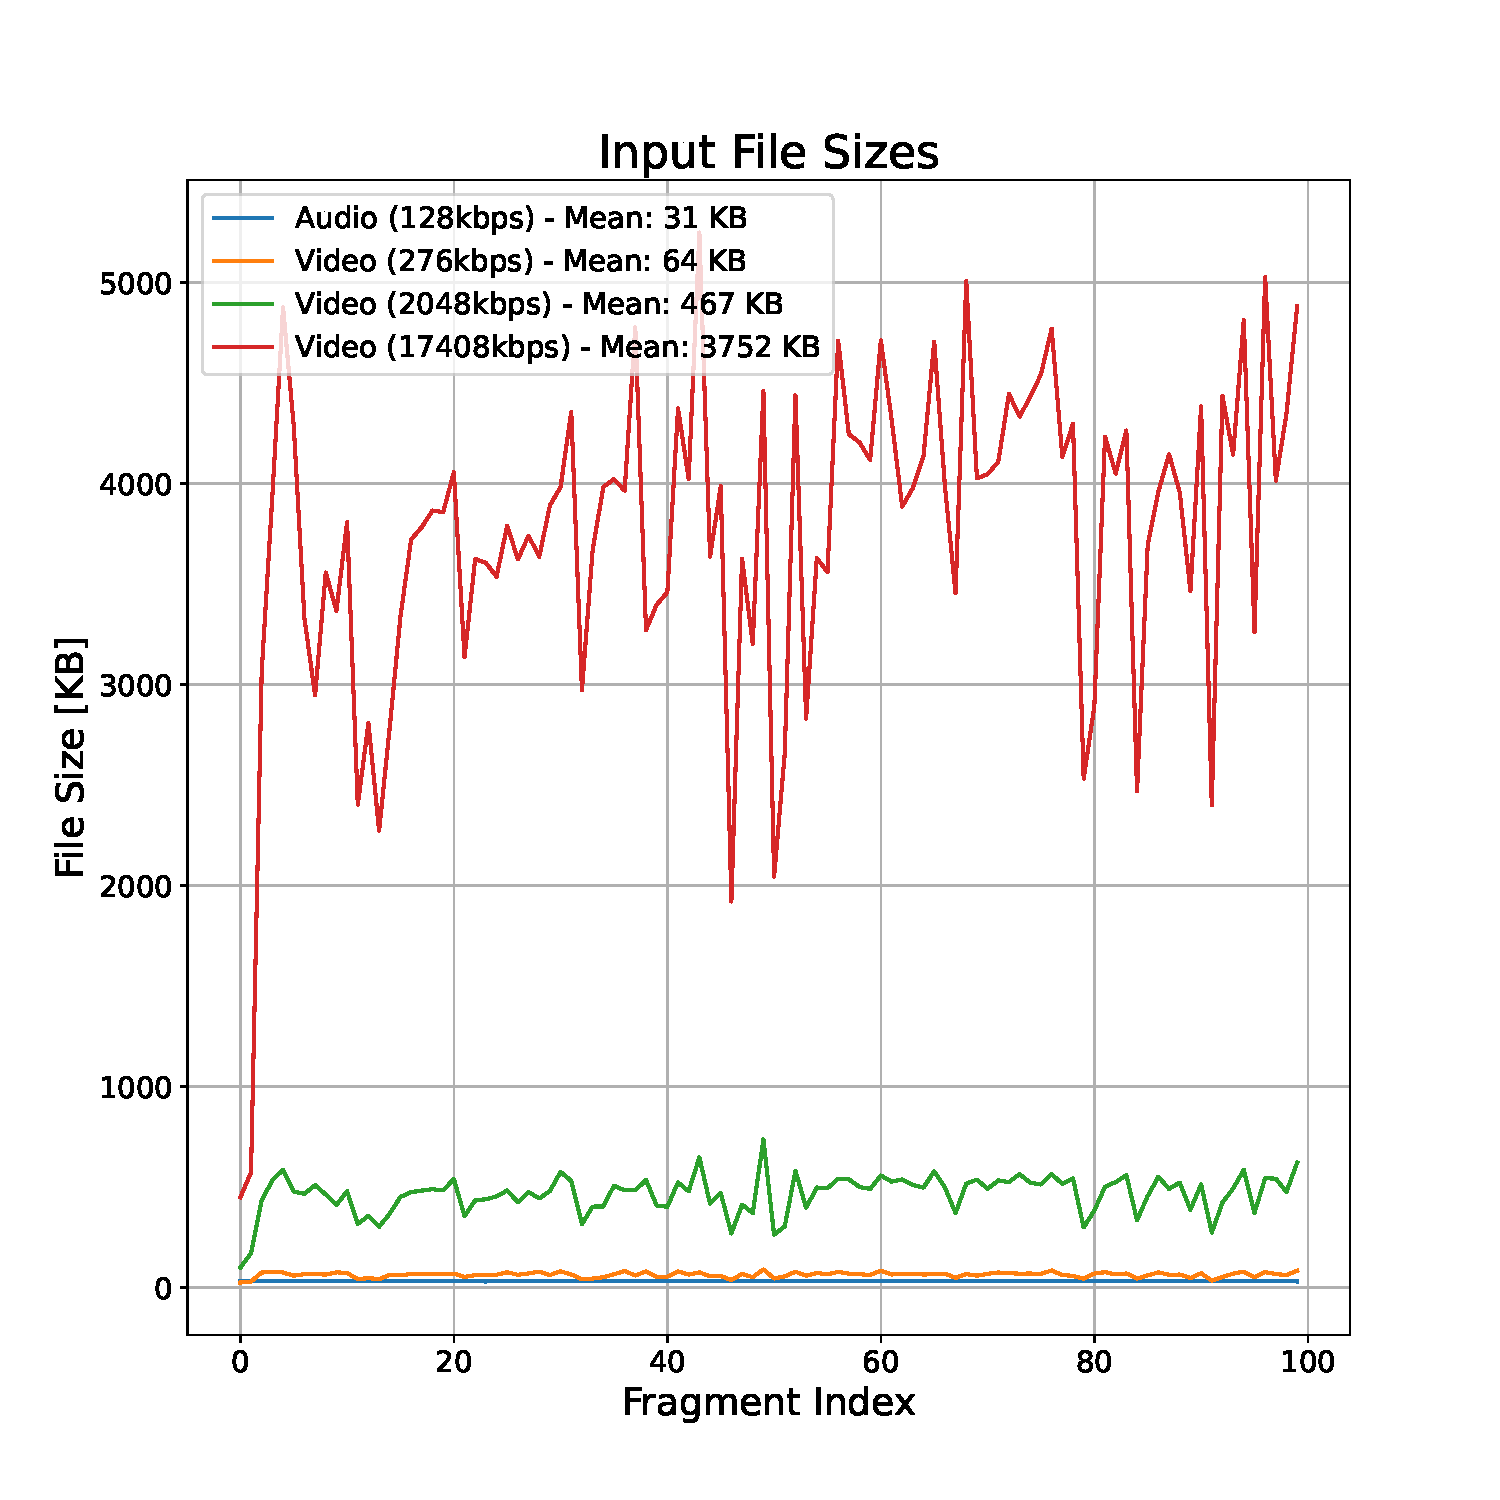
\includegraphics[width=0.75\linewidth]{plots/input-sizes.pdf}
    \caption{Input File Sizes}
    \label{fig:file-size}
\end{figure}

\subsection{Signing Duration}

In this benchmark I measured how long the entire signing function runs for to sign a live stream with up to 100 fragments. For this benchmark I loop through all available representations then for each signing method I iterate from 1 to 100 and sign the live stream at each index in accordance to the method. For the Rolling Hash signing this means that only the current fragments at that index is being signed. For the case of the optimized Merkle Tree approach I provide the signing function with the paths too all fragments up to the current index, but only the up to window size (eight) number of fragments are actually signed and for the original Merkle Tree every single fragment is being signed up to the current index.

The lower the time it takes to sign the newly created fragment, the less the impact on the streaming latency is, lower is better.

The time measuring can be described with the pseudo code from \Cref{alg:time-measure}. Essentially, I take a timestamp right before signing the fragments and right after the signing I take a second timestamp and the difference between the two timestamps is the time it took to sign the fragments. Then I save this value in a data structure in relation to the fragment index and representation the fragment belongs to.

\begin{algorithm}[H]
    \begin{algorithmic}[1]
        \State $now \gets Time.now()$
        \State sign\_fragments()
        \State $time \gets Time.since(now)$        
    \end{algorithmic}
    \caption{Duration Measuring Method}
    \label{alg:time-measure}
\end{algorithm}

In total I ran this benchmark ten times and averaged all results.

\subsection{Data Upload Size Required}

For this benchmark I looked at how much data has to be published to the CDN after each fragment has been signed. I measured this by simply adding up the file sizes of all the files that were affected by the signing of the current fragment, which would subsequently be needed to be uploaded to the CDN. In case of the Rolling Hash approach that is only the initialization fragment and the fragment at the current index. For the optimized Merkle Tree approach that is the initialization fragment and all fragments of the current Merkle Tree, which are up to eight fragments with my configuration and again all fragments for the original Merkle Tree signing. The original Merkle Tree signing requires to upload every single fragmnet up to the current index.

Since this benchmark is merely adding up file sizes I ran this one in conjunction with the previous duration benchmark, so I don't have to sign everything multiple times for each benchmark.

In this benchmark a lower upload size equals to less overhead on the network and a better caching situation for the CDN, again lower is better.

\section{Performance Measurements\label{sec:performance}}

In this section I will present the results of the above described benchmarks and give my evaluation and observations about them.

\subsection{Signing Duration}

I have split the data plots into two comparisons. One comparing each signing method in relation to the different representations, shown in \Cref{fig:sign-dur1} and the other comparing the signing method to each other per representation, shown in \Cref{fig:sign-dur2}.

This signing procedure is the added step into the creation of this live stream which is why I equate the signing duration as the impact on the latency of the live stream.

Since the original Merkle Tree signing method signs every single fragment that has been created over the course of the live stream, I expected the overall signing duration to steadily increase as the live stream gets longer. This expectation is confirmed when looking at \Cref{fig:sign-dur1-og}. The signing duration of all four representations linearly increases in proportion to the number of fragments that are being included in the signing process. It can also be deduced that the larger the input files are the stronger the duration increases. 

I will score the performance of the original Merkle Tree signing method by looking at how many fragments can be signed within one second. Since the graphs are consistently linear, I will measure this score by taking the signing duration of the 100th fragment and extrapolating its signing duration to one second.

The audio representation has the lowest signing duration of all, which is expected since it also has the lowest input file sizes with an average of \texttt{31 kilobyte}. The score of this representation is \texttt{528} fragments, which can be signed within one second. The next fastest signing duration is the low video representations with an average file size of \texttt{64 kilobyte}. The score of this representation is \texttt{344} fragments. The mid video representation has the second slowest signing duration with average file sizes of \texttt{467 kilobyte} and a score of \texttt{82} fragment. The slowest signing duration is expectedly measured on the high video representation with average file sizes of \texttt{3,752 kilobyte} and a score of only \texttt{13} fragments.

The optimized Merkle Tree signing method uses essentially the same concepts of the original equivalent but with the added constraint that eight fragments are grouped into separate Merkle Trees. The expectations of this method is that the signing duration will look very similar for each individual Merkle Tree but reset every eight fragments. The plot in \Cref{fig:sign-dur1-opt} confirm this expectation.

The plot perfectly shows the sawtooth-signal-like graph of this approach. It starts with a low signing duration then it increases linearly like the original method and then peaks at every eighth fragment before it resets back down to the low duration. The important metric of this approach are the extreme signing durations, by which I will score the individual representations.

The order slowest to fastest is the same as before. The audio representation is the fastest with a minimum signing duration around \texttt{8} milliseconds and a peak of \texttt{25} milliseconds. Again followed by the low video representation with a minimum duration of about \texttt{8} milliseconds and a peak of roughly \texttt{35} milliseconds. The next slowest is the mid video representation with the low point signing duration being on average \texttt{10} milliseconds and a maximum of around \texttt{100} milliseconds. The slowest is again the high video representation with minimum signing duration about \texttt{100} milliseconds and peaks up to \texttt{700} milliseconds.

Looking at the plot of the Rolling Hash signing method in \Cref{fig:sign-dur1-rh} is clear that this is fast method overall by a good margin. Since this approach only every signs the current fragment, the signing duration directly correlates to the input file size. The three lowest representation have near constant signing duration. The audio presentation has an average of \texttt{10.5} milliseconds. The video low and mid video representations have average signing duration of \texttt{11.8} and \texttt{21.3} milliseconds, respectively. The high video representation fluctuates a lot more than the other representations but the majority of the time it remains in roughly the same interval between \texttt{80} and \texttt{100} milliseconds with an overall average of \texttt{86.5} milliseconds. When looking at the plots of \Cref{fig:sign-dur1-rh} and \Cref{fig:file-size} side by side, it is very obvious that these results are expected. The files sizes for the lower representations line up the with stability of the signing duration and the fluctuation of the higher representations equally lines up with the signing durations.

\begin{figure}
    \centering
    \subfloat[Original Merkle Tree]{
        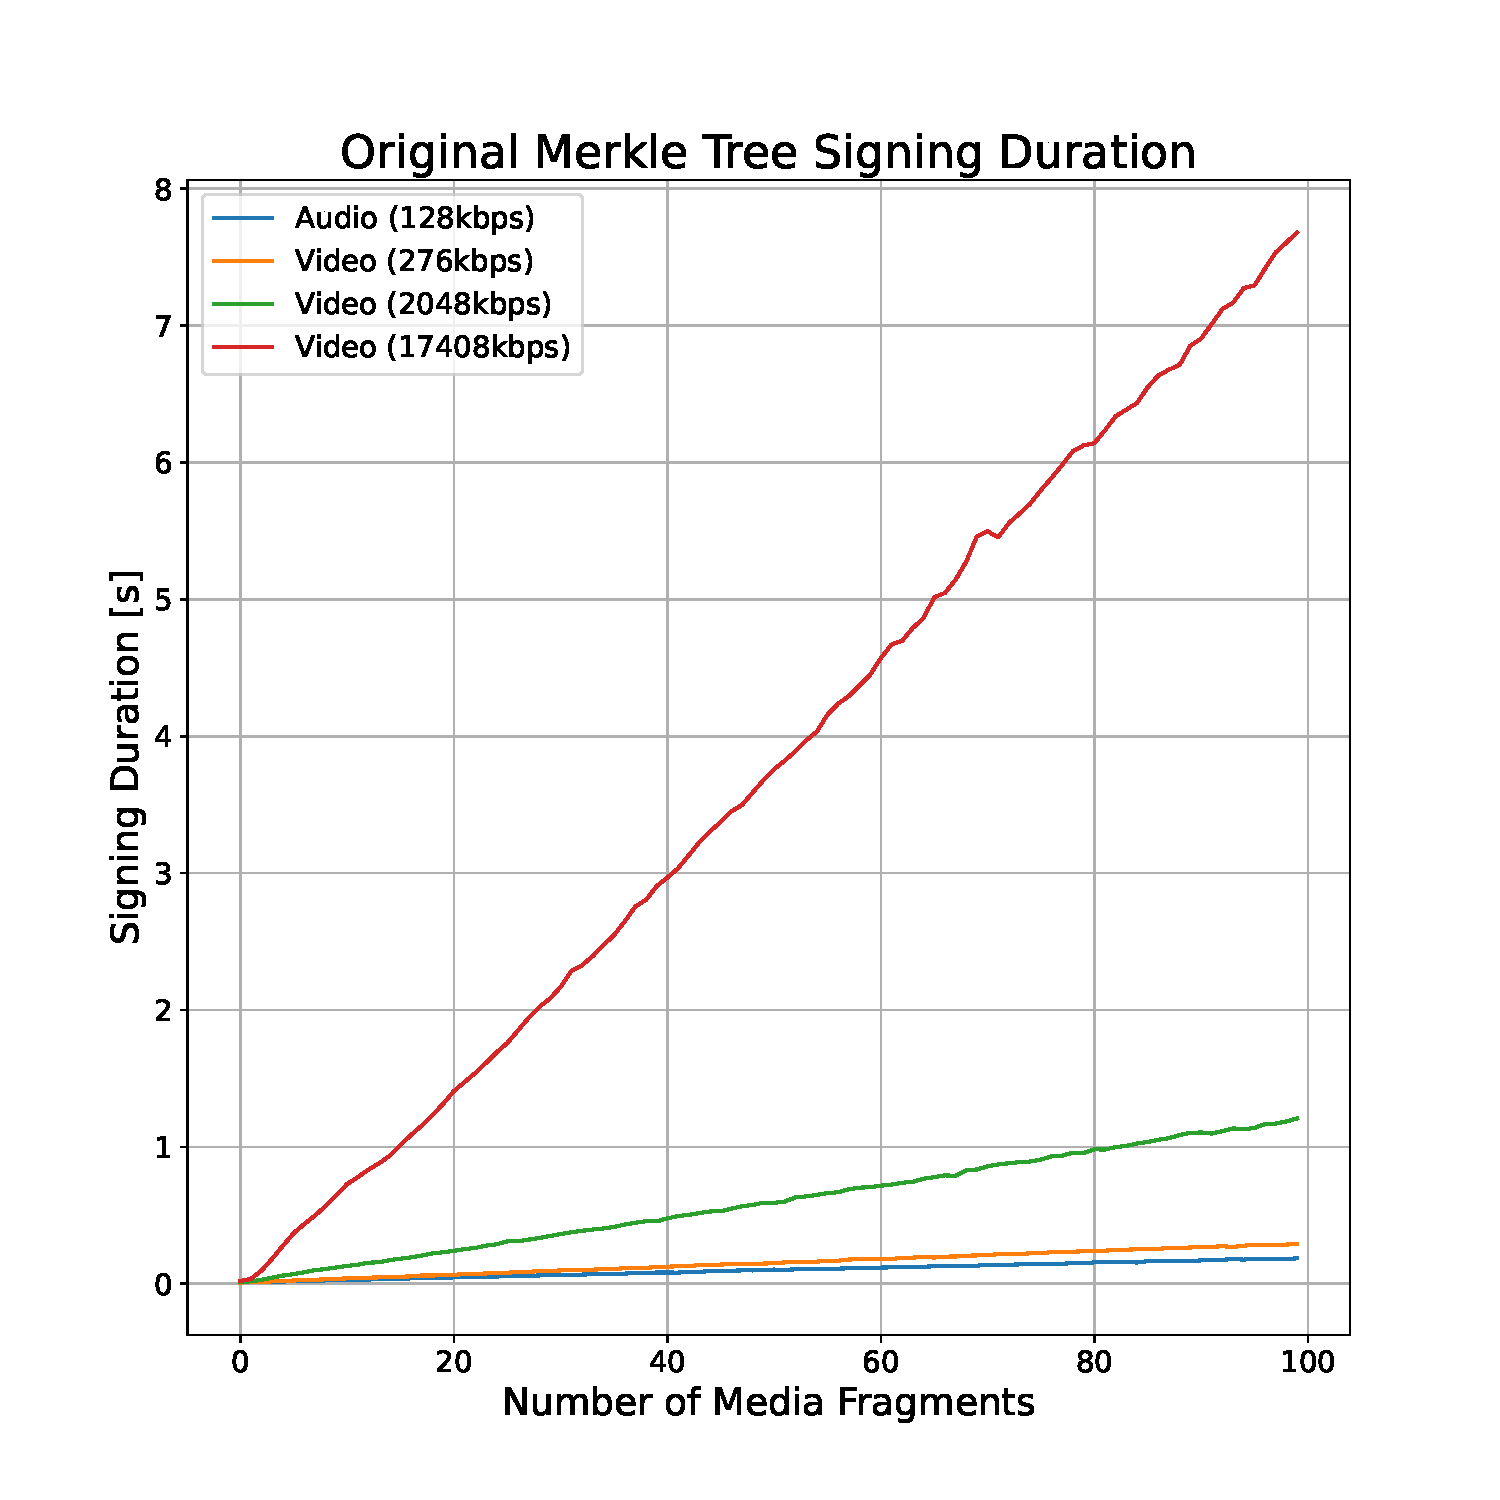
\includegraphics[width=0.49\linewidth]{plots/time-original-merkle-tree.pdf}
        \label{fig:sign-dur1-og}
    }
    \subfloat[Optimized Merkle Tree]{
        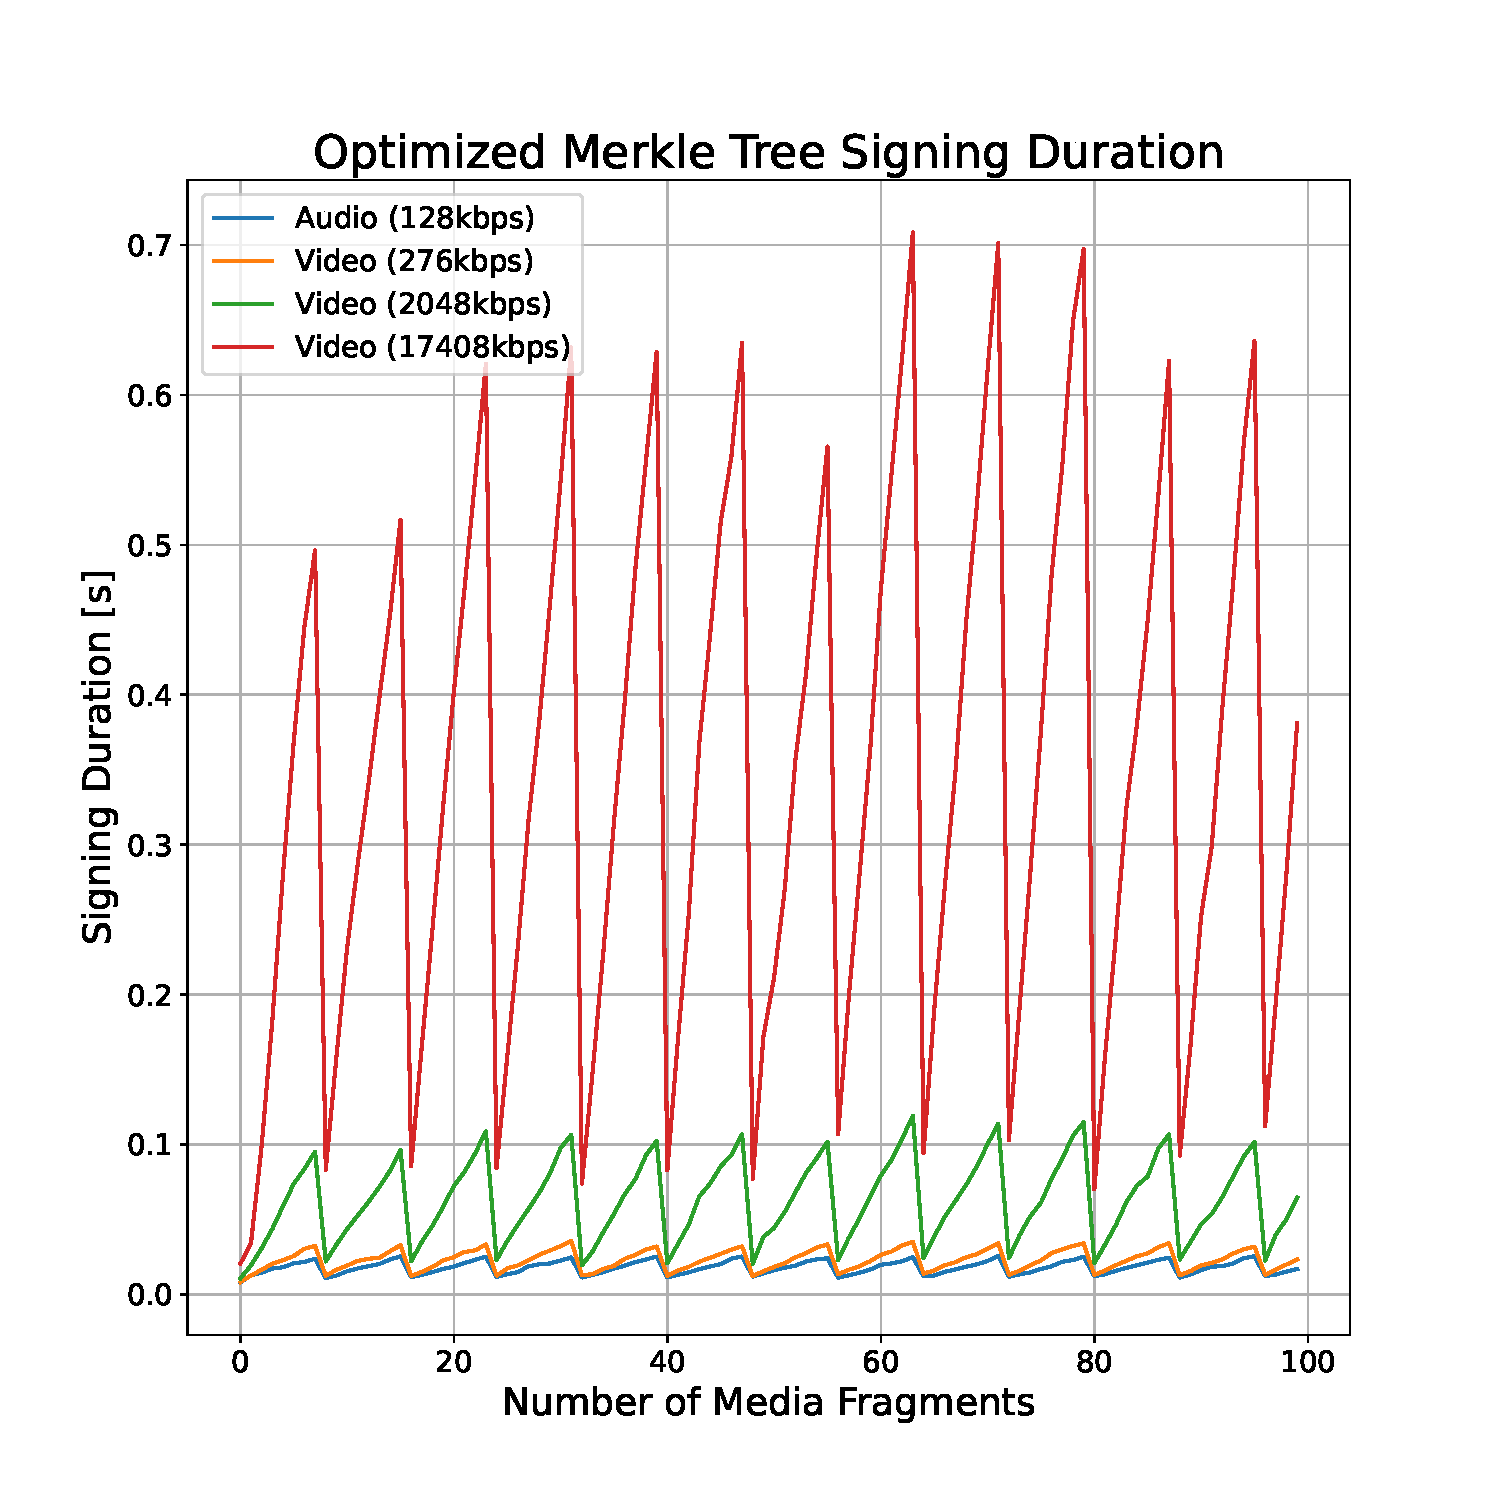
\includegraphics[width=0.49\linewidth]{plots/time-optimized-merkle-tree.pdf}
        \label{fig:sign-dur1-opt}
    } \\
    \subfloat[Rolling Hash]{
        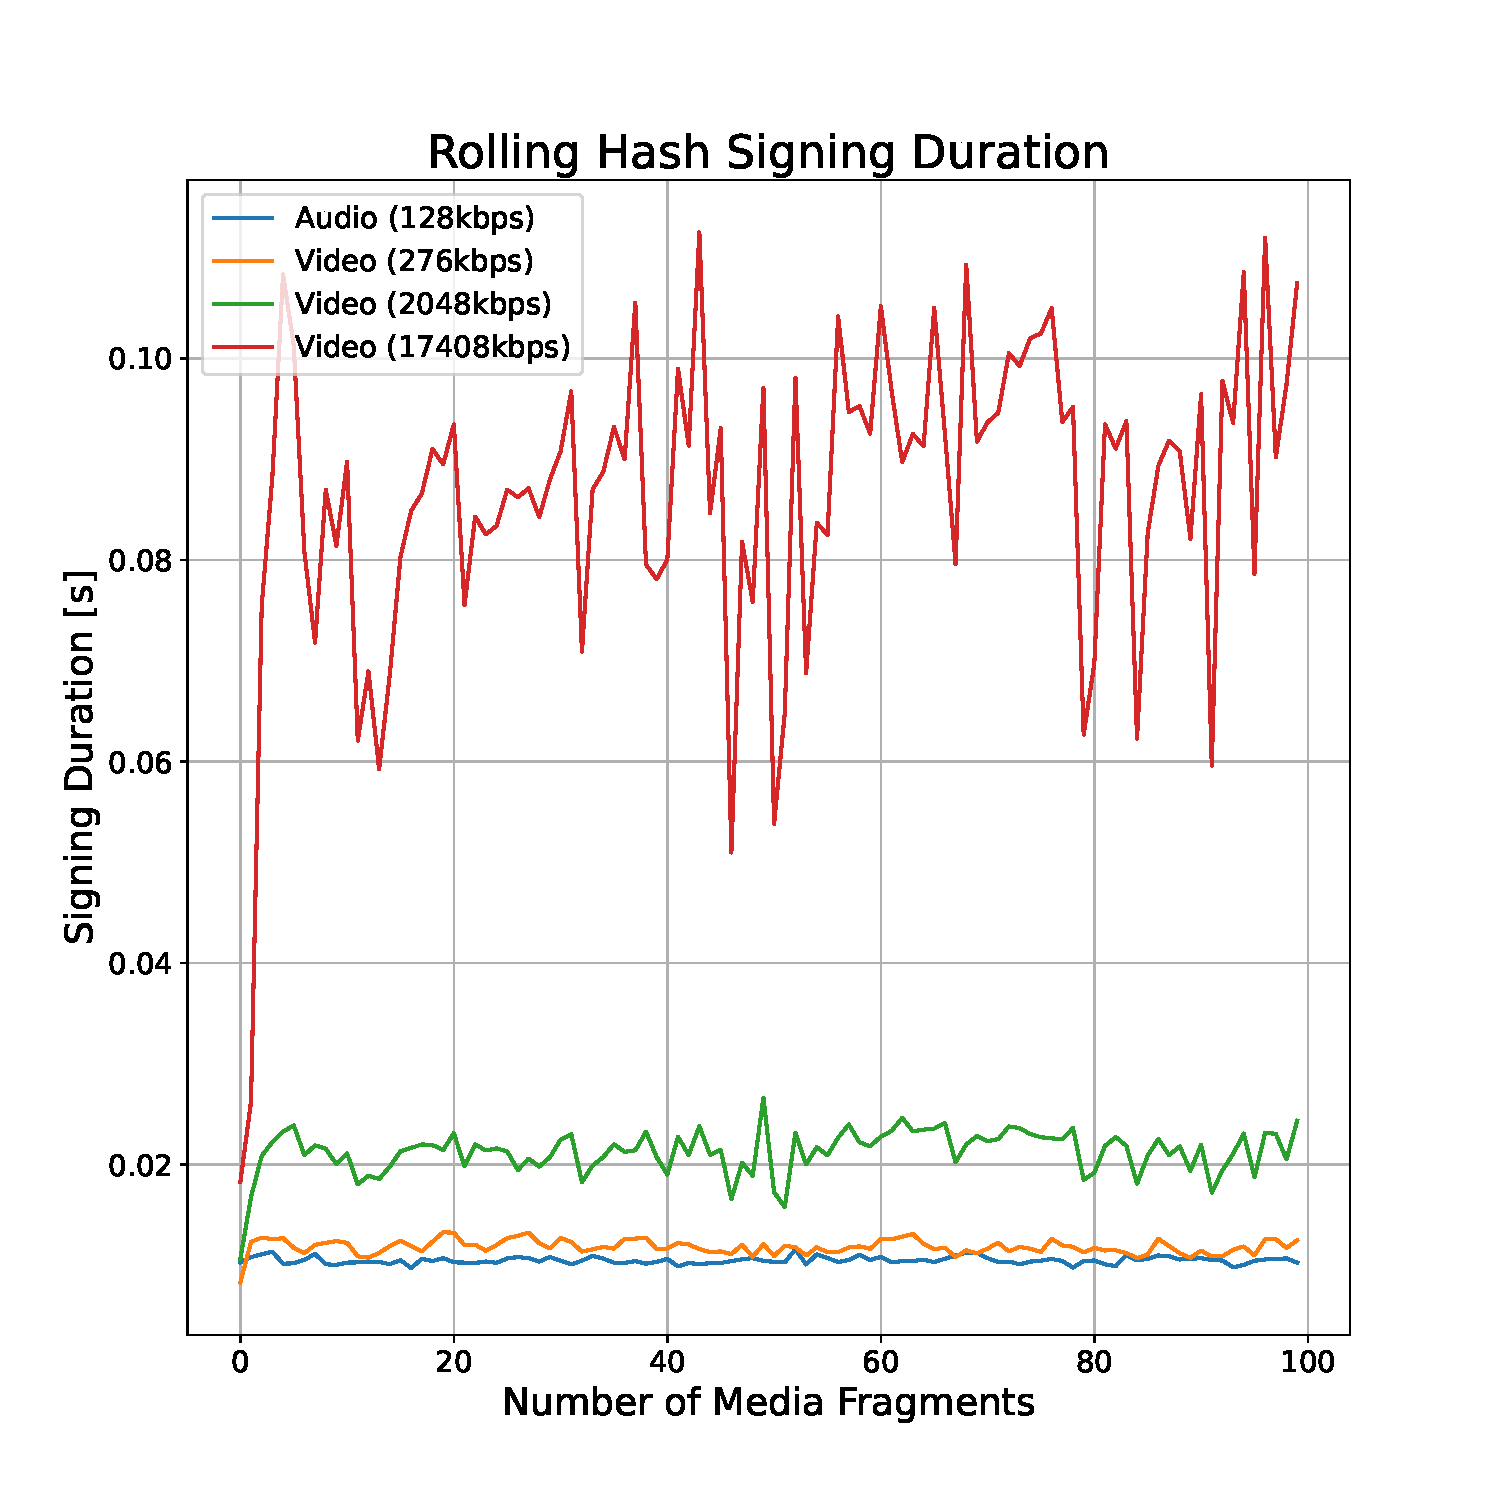
\includegraphics[width=0.49\linewidth]{plots/time-rolling-hash.pdf}
        \label{fig:sign-dur1-rh}
    }
    \caption{Signing Duration Results}
    \label{fig:sign-dur1}
\end{figure}

Now looking at the comparison of the signing methods to each other in \Cref{fig:sign-dur2}, it gets directly apparent that the signing methods all perform essentially the same in regards to what representation is being signed. However, these plots show very well that the original signing method is by a large margin the slowest signing method, with the optimized Merkle Tree signing method being much more competitive with the Rolling Hash method but the Rolling Hash method is still the best.

\begin{figure}
    \centering
    \subfloat[Audio (128kbps)]{
        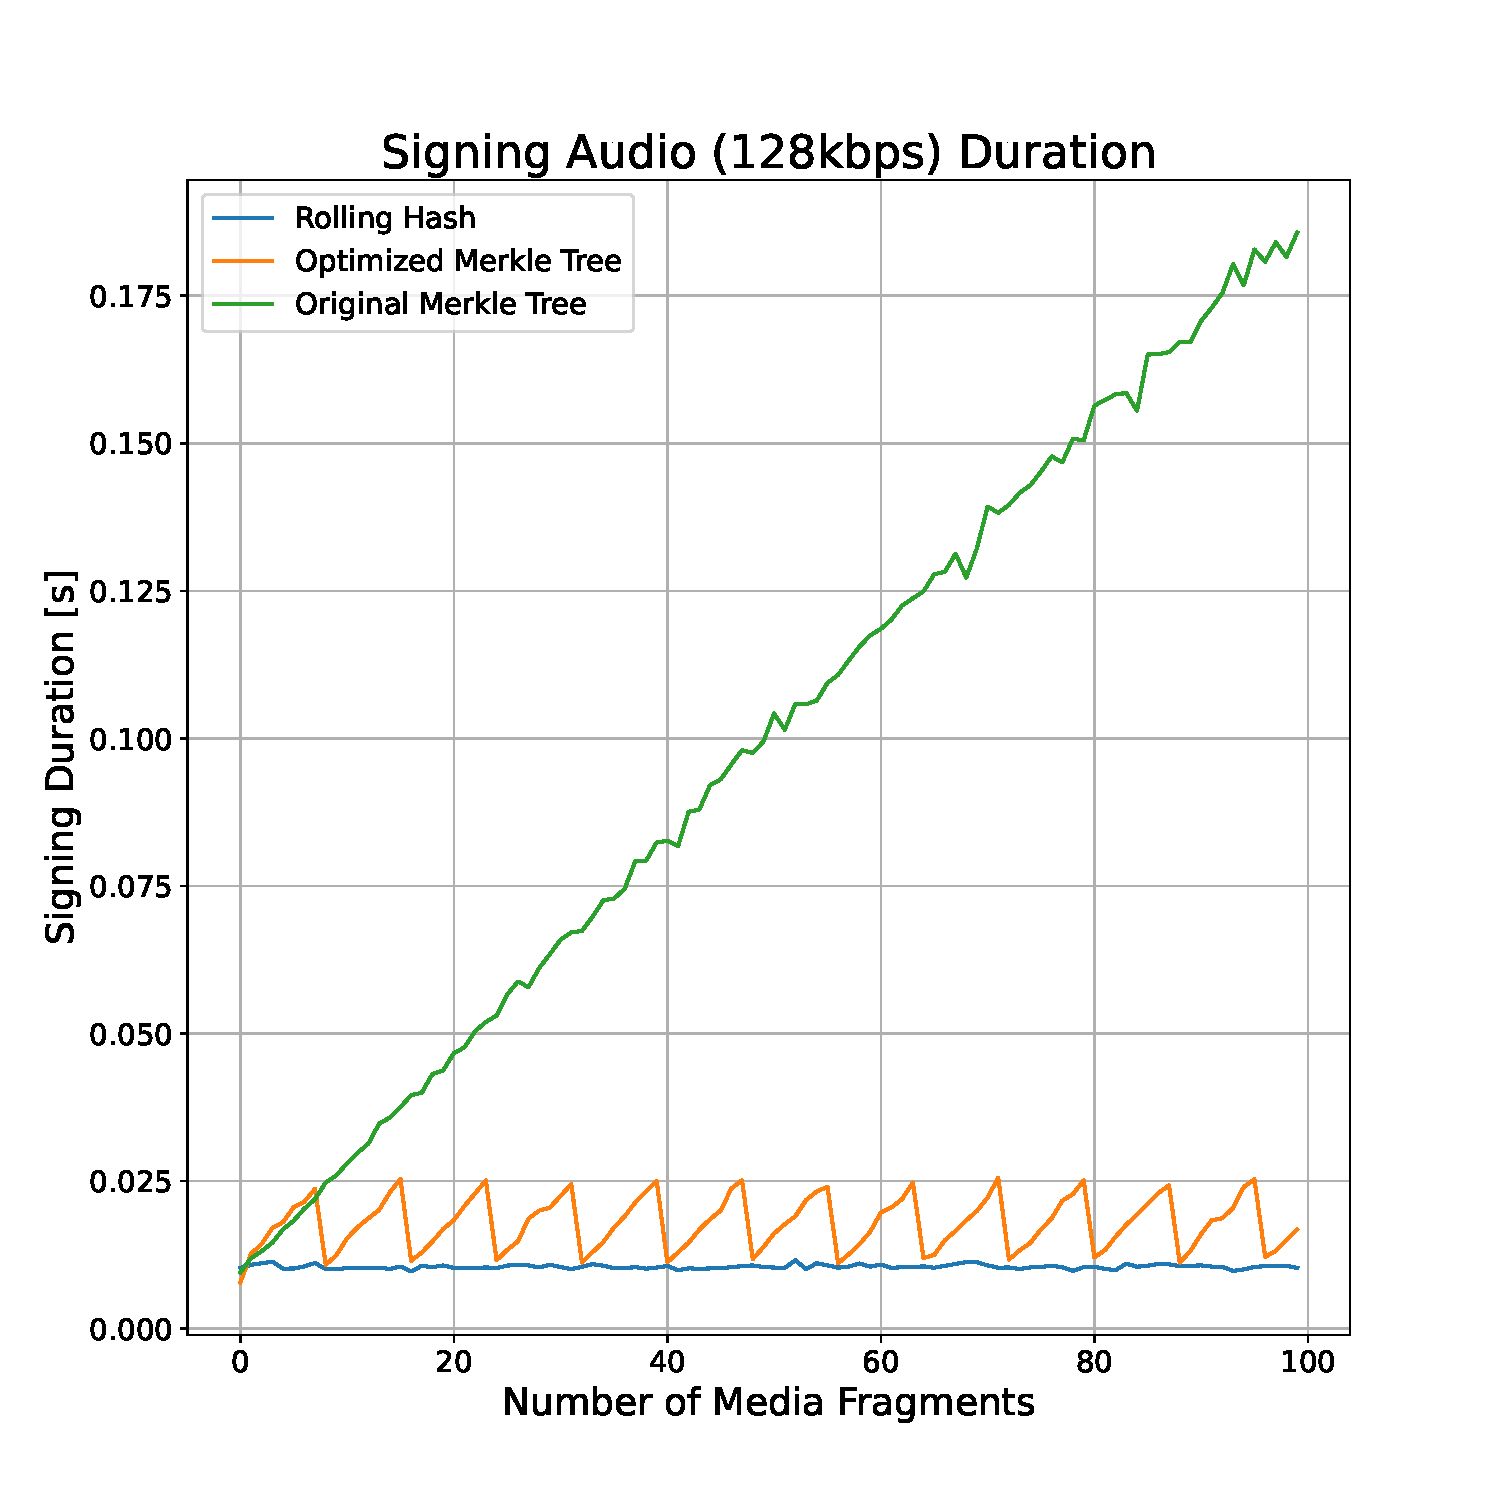
\includegraphics[width=0.49\linewidth]{plots/compare-time-Audio-(128kbps).pdf}
        \label{fig:sign-dur2-audio}
    }
    \subfloat[Video (276kbps)]{
        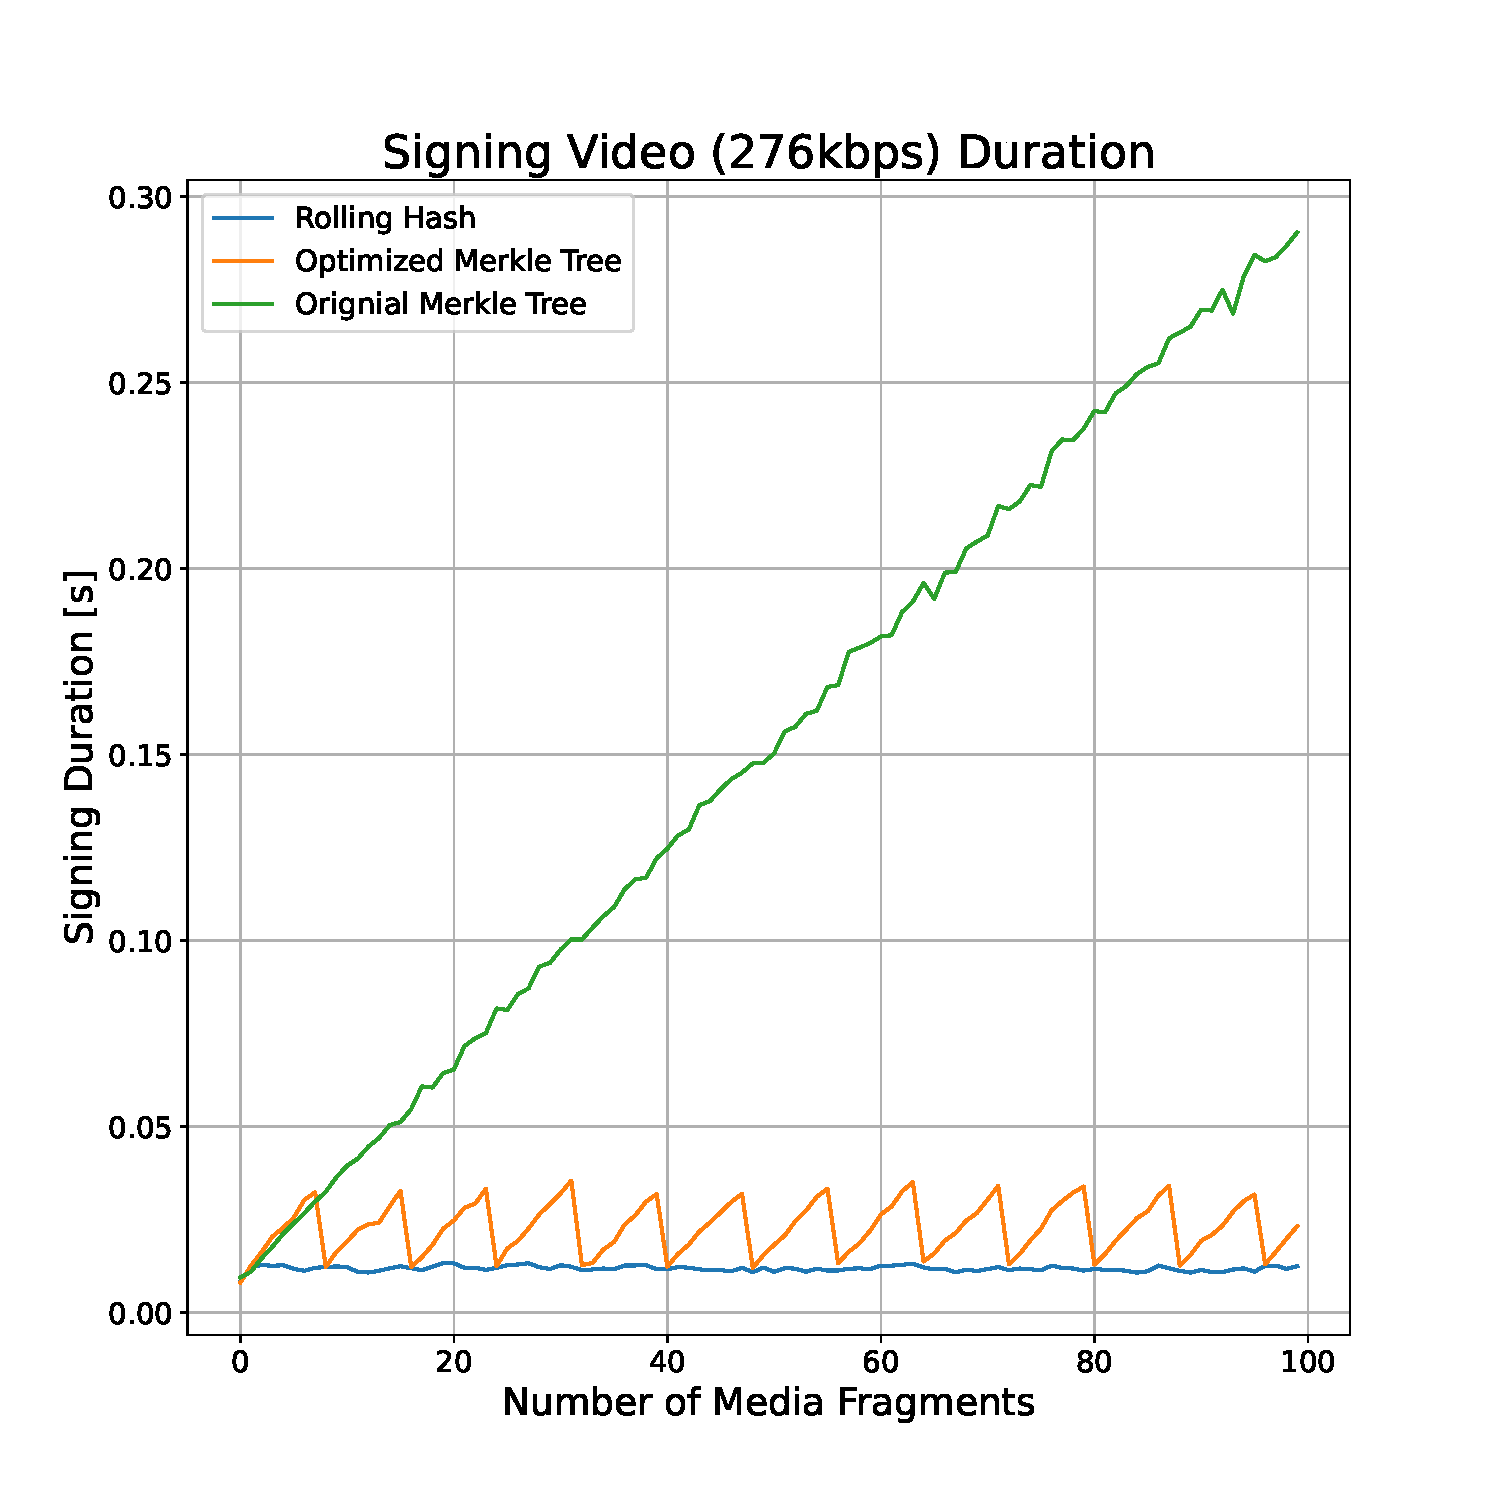
\includegraphics[width=0.49\linewidth]{plots/compare-time-Video-(276kbps).pdf}
        \label{fig:sign-dur2-video1}
    } \\
    \subfloat[Video (2,048kbps)]{
        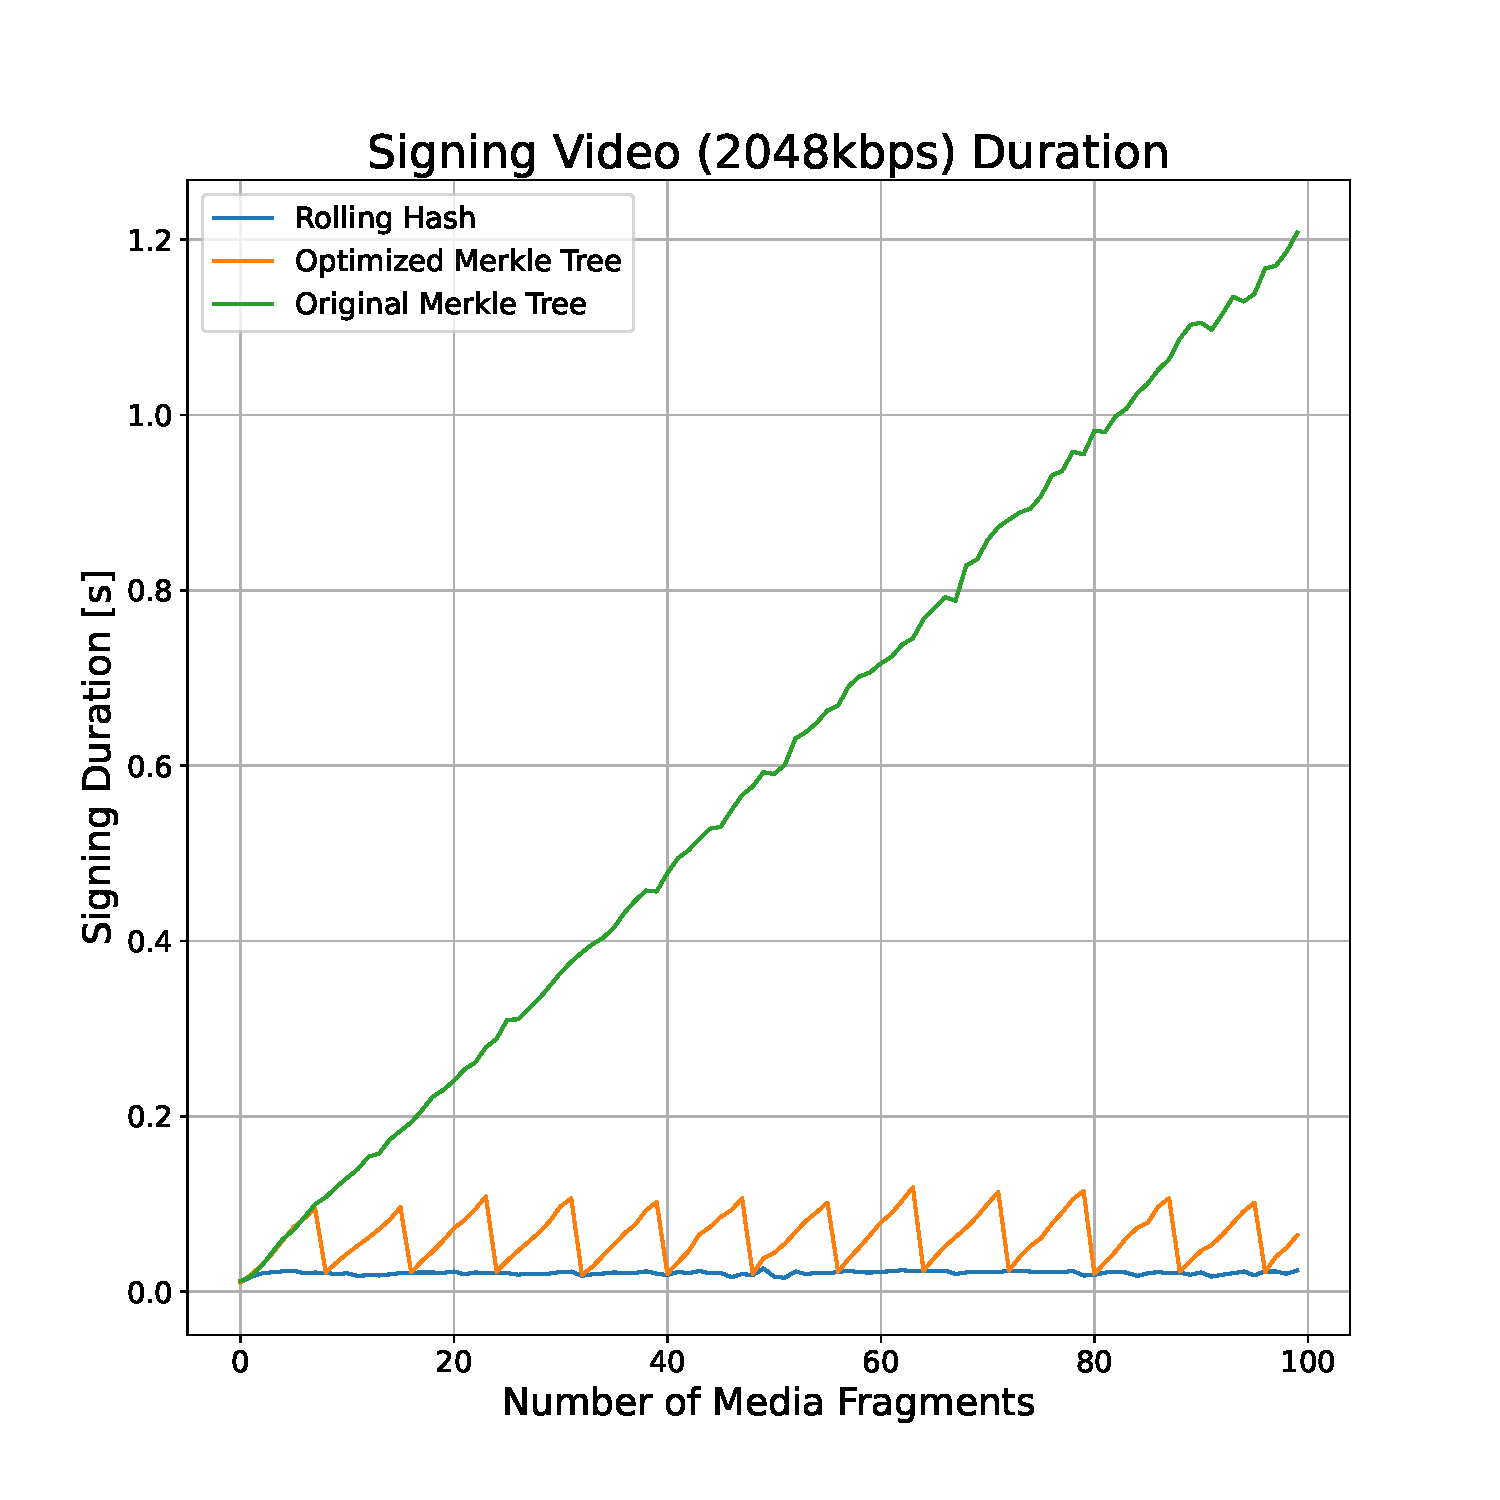
\includegraphics[width=0.49\linewidth]{plots/compare-time-Video-(2048kbps).pdf}
        \label{fig:sign-dur2-video2}
    }
    \subfloat[Video (17,408kbps)]{
        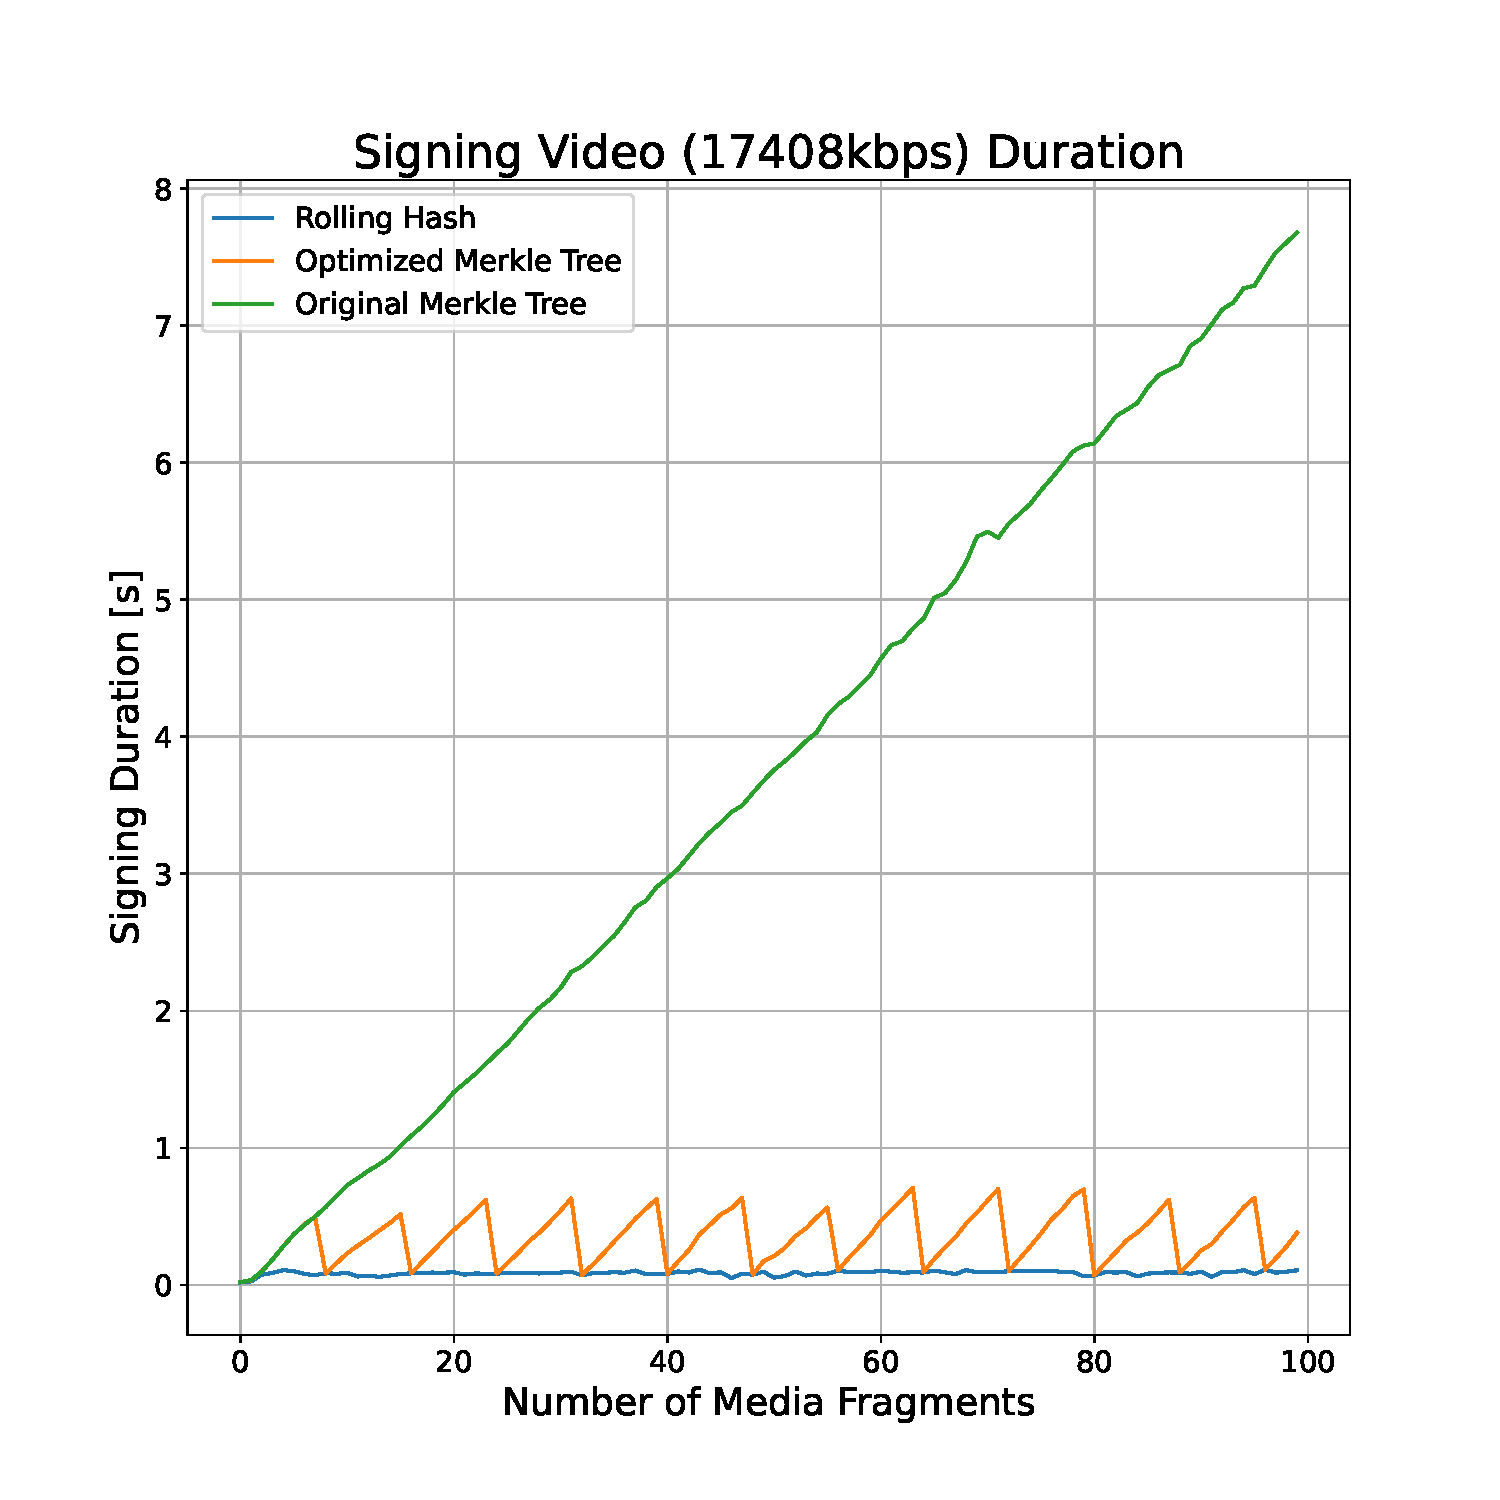
\includegraphics[width=0.49\linewidth]{plots/compare-time-Video-(17408kbps).pdf}
        \label{fig:sign-dur2-video3}
    }
    \caption{Signing Duration Results}
    \label{fig:sign-dur2}
\end{figure}

\subsection{Data Upload Size Required}

For this benchmark I have split the data plots into the same comparisons as before: comparing each signing method in relation to the different representations are shown in \Cref{fig:upload1} and the signing methods compared to each other per representation are shown in \Cref{fig:upload2}.

In essence, the results of the required data upload size is exactly the same as the signing duration benchmark. The original Merkle Tree method requires by far the most data upload, of which the majority is entirely redundant, because every time a new fragment is being signed, every single prior fragment is being signed as well and subsequently they have to be published anew to the CDN to have the most up-to-date data available. As before it also shows a linear increase as the number of fragment rises. All the representations have an gradient of slightly more then the average file size per fragment, as shown in \Cref{fig:file-size}. The reason by this is that with every new fragment everything from before has to be uploaded again, as already mentioned and the gradient is a little more because the added C2PA data is now included in the files. These results are shown in \Cref{fig:upload1-og}.

The same goes for the optimized Merkle Tree signing approach, shown in \Cref{fig:upload1-opt}. Again a sawtooth-signal-like graph can be observed which resets every eighth fragment. In all cases the needed upload is considerably lower than compared to the original method.

Lastly, the Rolling Hash results are equally the same, as seen in \Cref{fig:upload1-rh}. The three lower representations again have a near constant value and the highest fluctuates slightly but overall still significantly lower than the other two methods.

\begin{figure}
    \centering
    \subfloat[Original Merkle Tree]{
        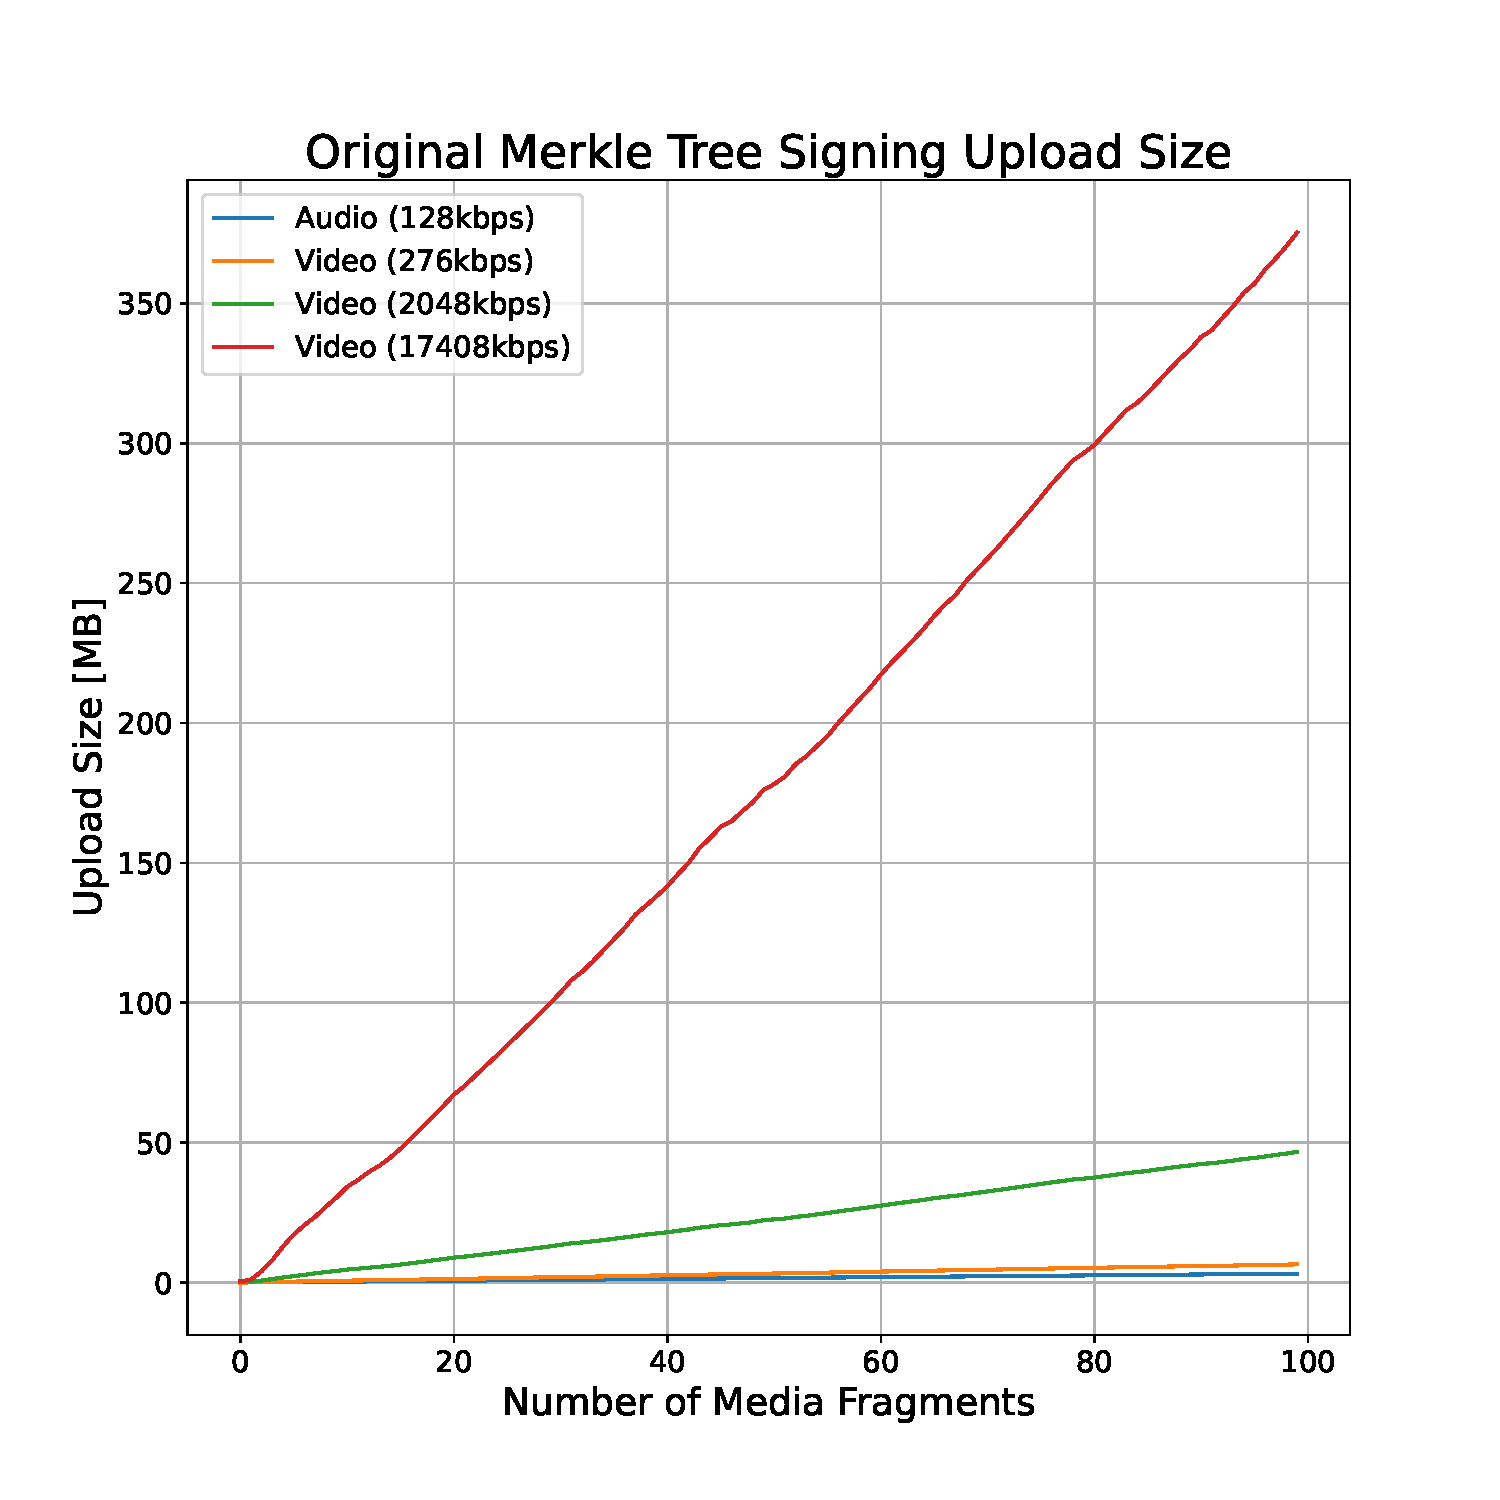
\includegraphics[width=0.49\linewidth]{plots/upload-original-merkle-tree.pdf}
        \label{fig:upload1-og}
    }
    \subfloat[Optimized Merkle Tree]{
        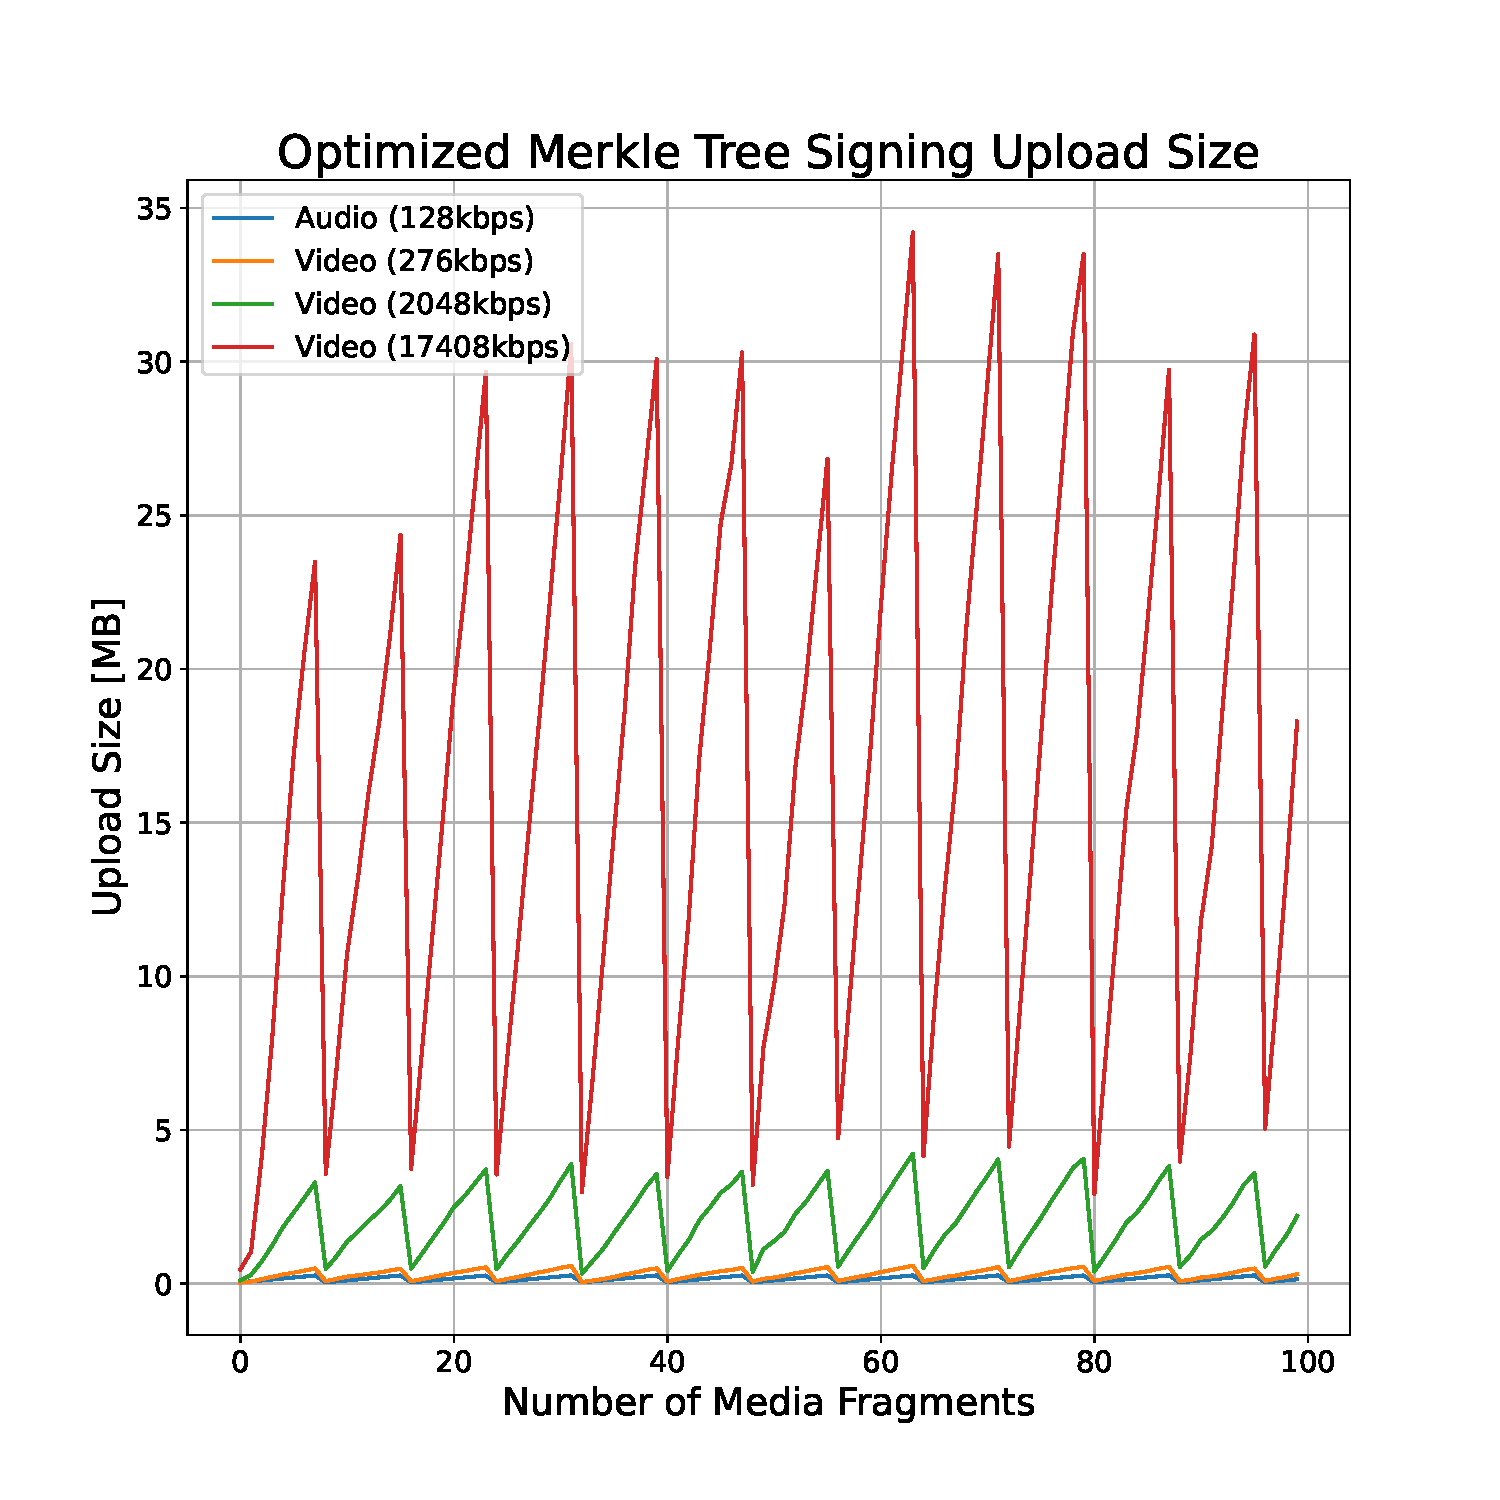
\includegraphics[width=0.49\linewidth]{plots/upload-optimized-merkle-tree.pdf}
        \label{fig:upload1-opt}
    } \\
    \subfloat[Rolling Hash]{
        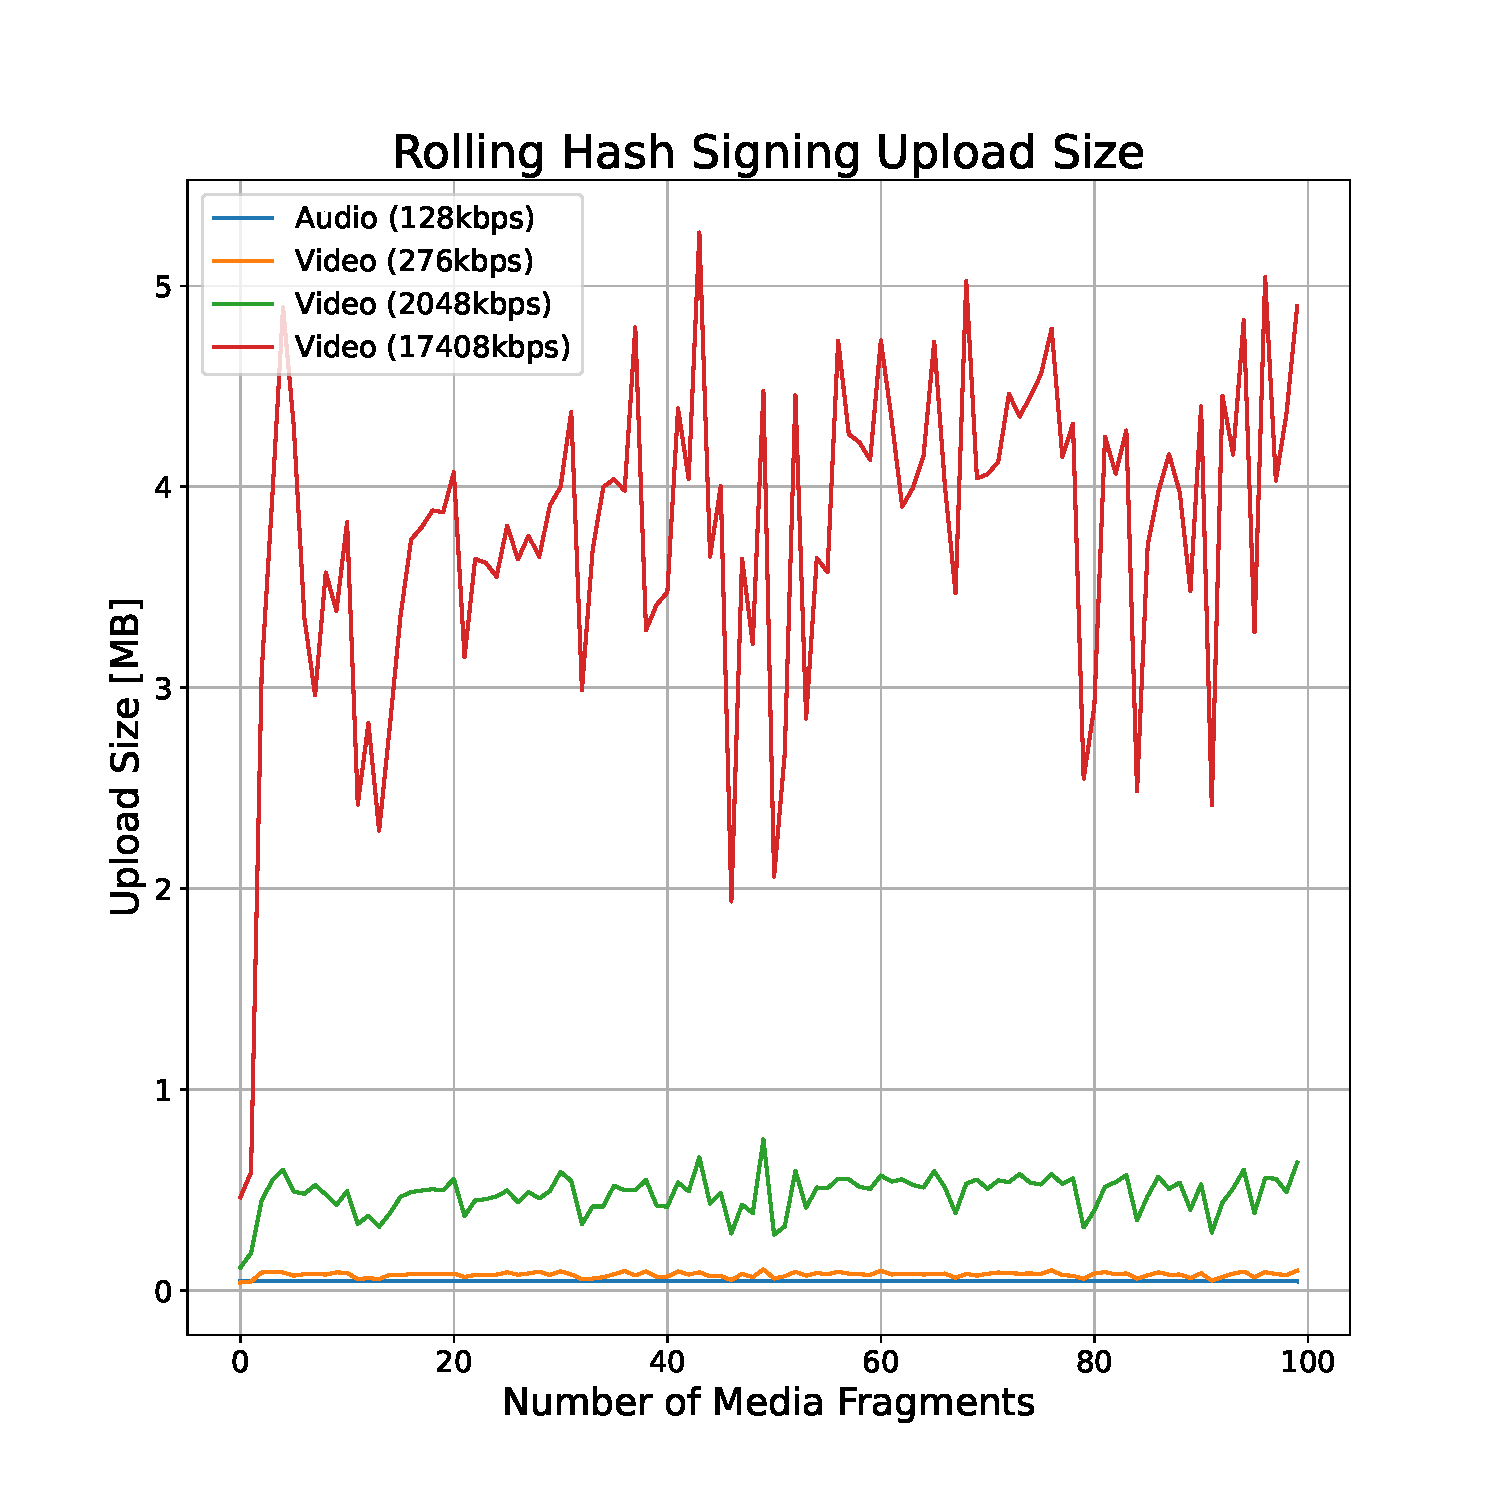
\includegraphics[width=0.49\linewidth]{plots/upload-rolling-hash.pdf}
        \label{fig:upload1-rh}
    }
    \caption{Upload Size Results}
    \label{fig:upload1}
\end{figure}

\begin{figure}
    \centering
    \subfloat[Audio (128kbps)]{
        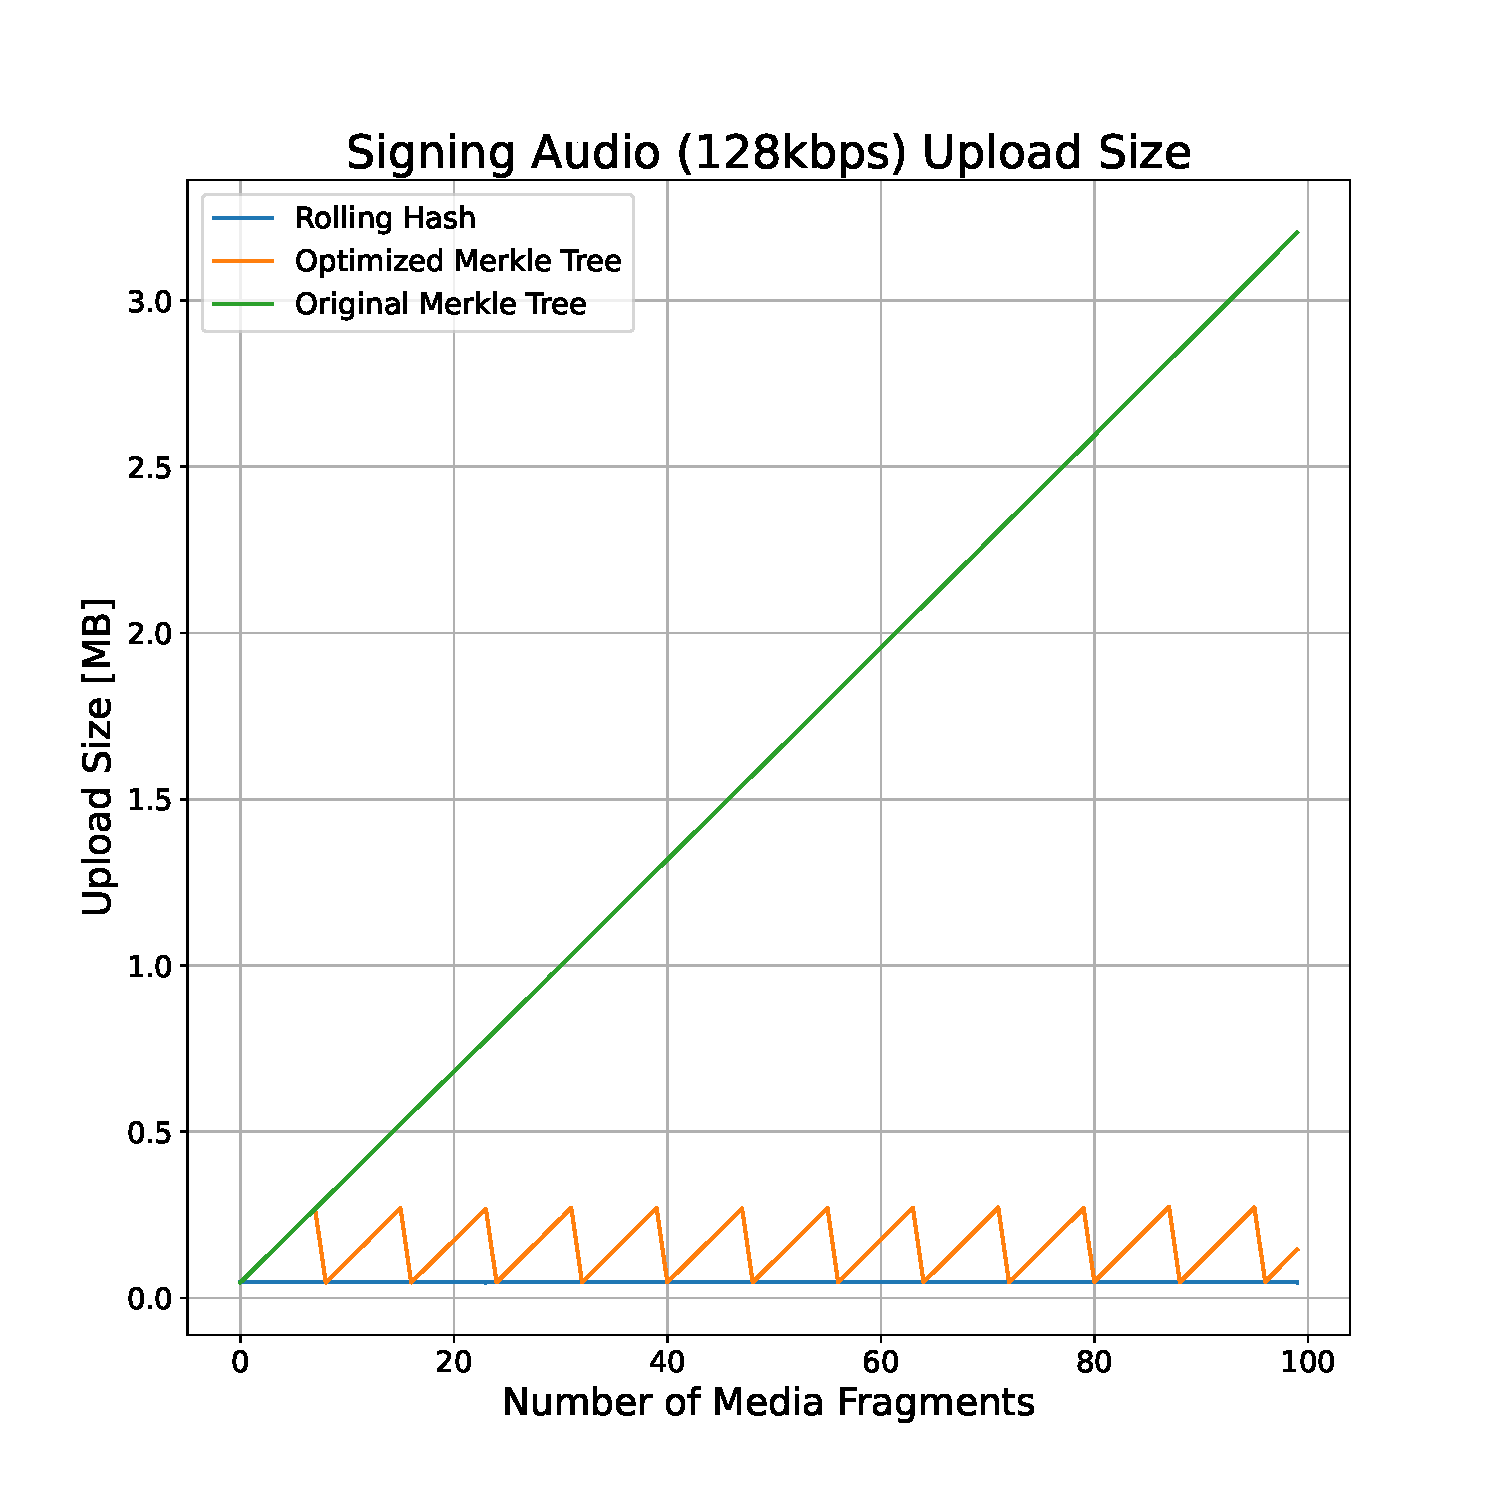
\includegraphics[width=0.49\linewidth]{plots/compare-upload-Audio-(128kbps).pdf}
        \label{fig:upload2-audio}
    }
    \subfloat[Video (276kbps)]{
        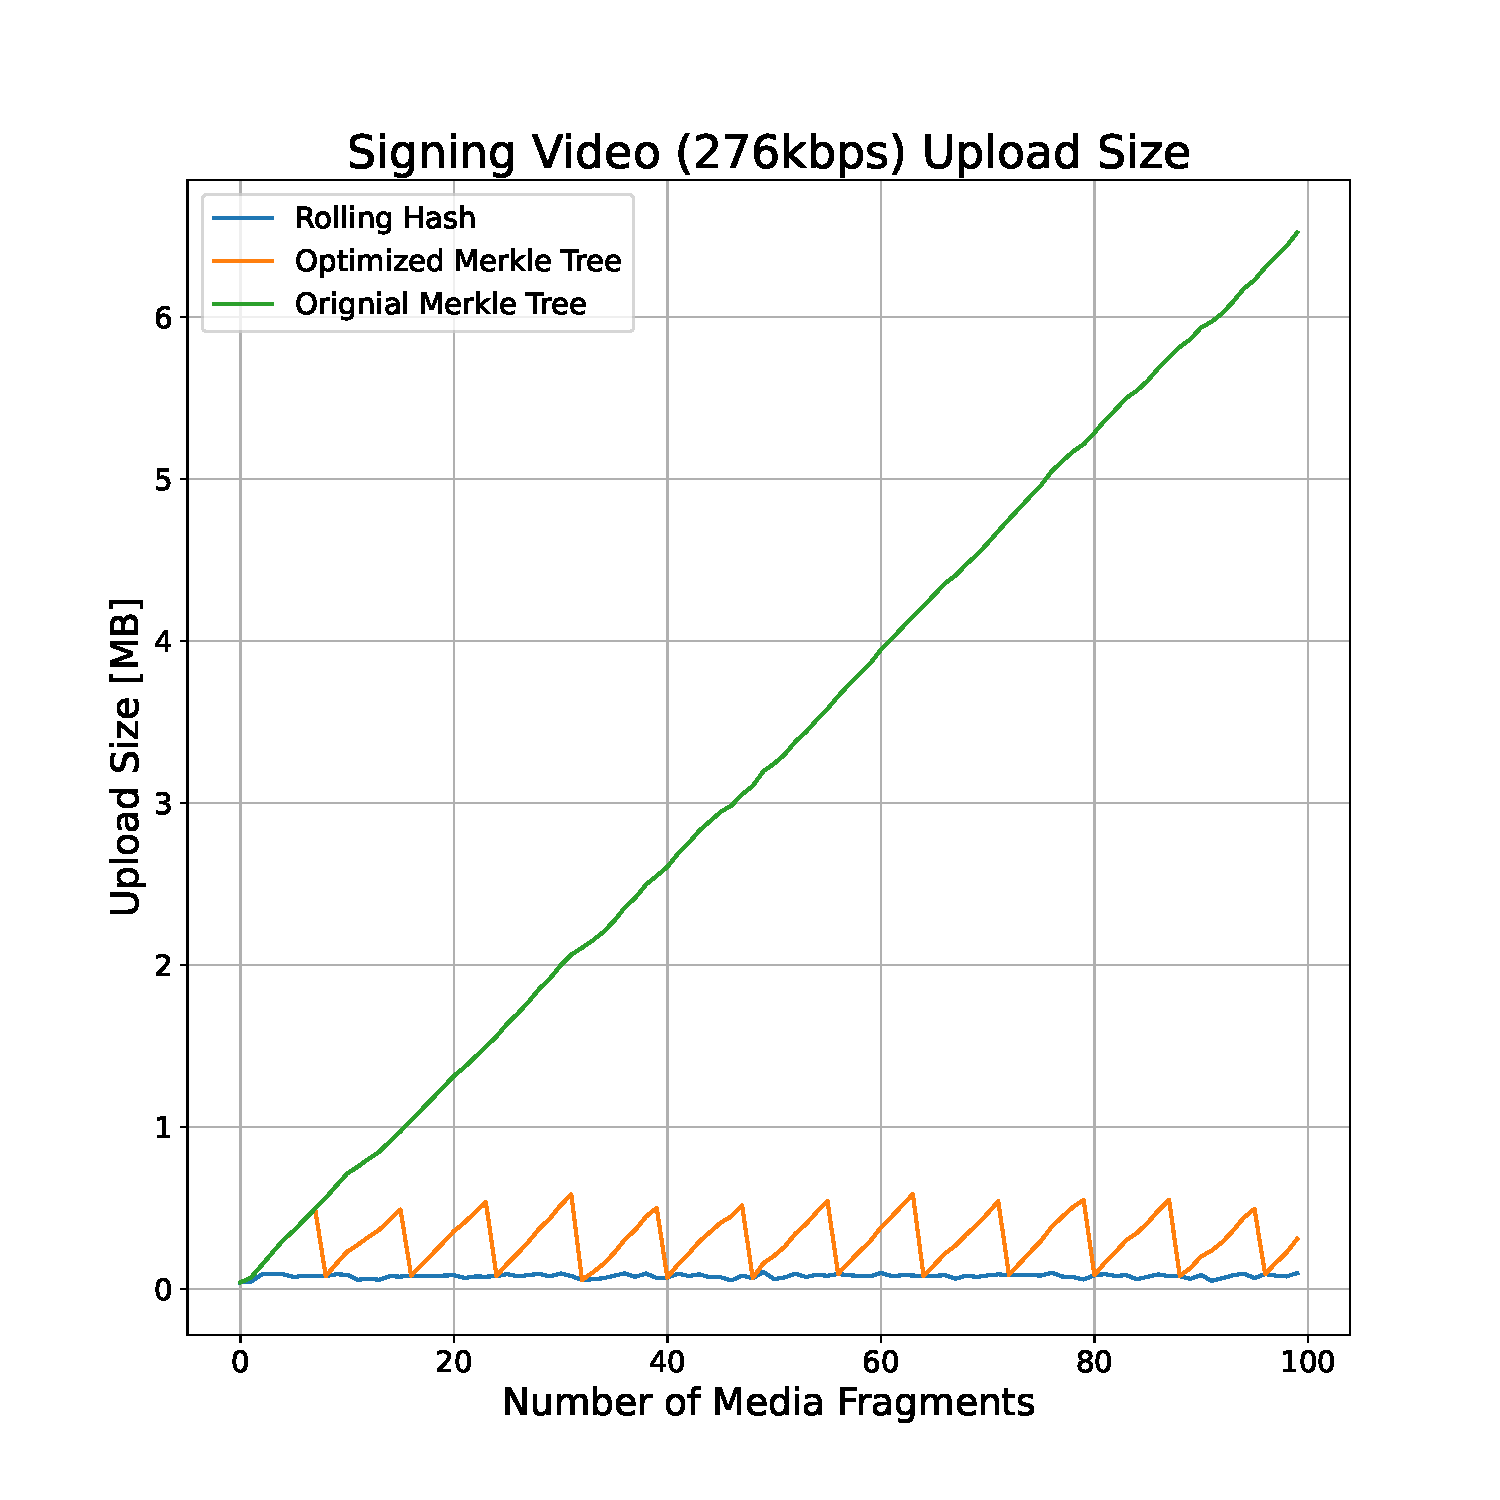
\includegraphics[width=0.49\linewidth]{plots/compare-upload-Video-(276kbps).pdf}
        \label{fig:upload2-video1}
    } \\
    \subfloat[Video (2,048kbps)]{
        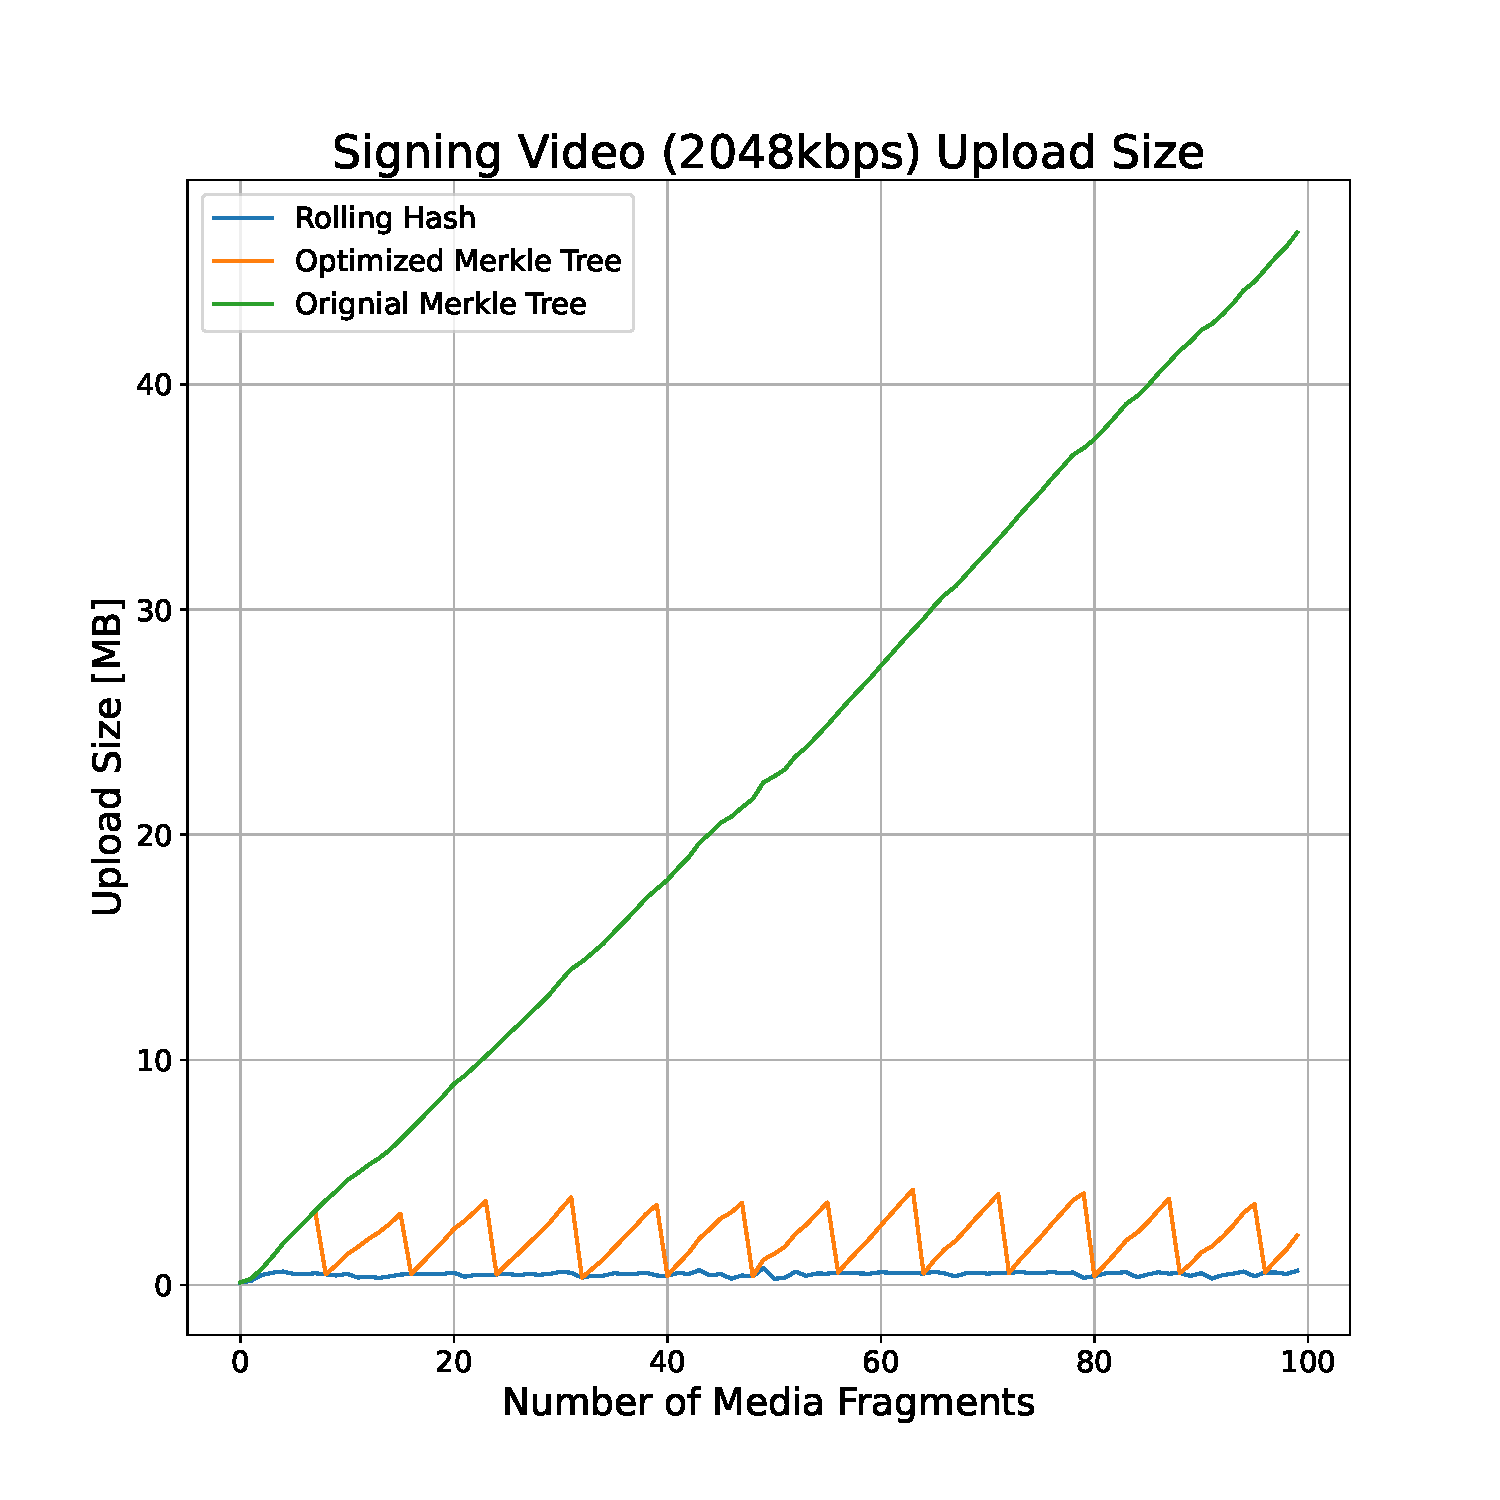
\includegraphics[width=0.49\linewidth]{plots/compare-upload-Video-(2048kbps).pdf}
        \label{fig:upload2-video2}
    }
    \subfloat[Video (17,408kbps)]{
        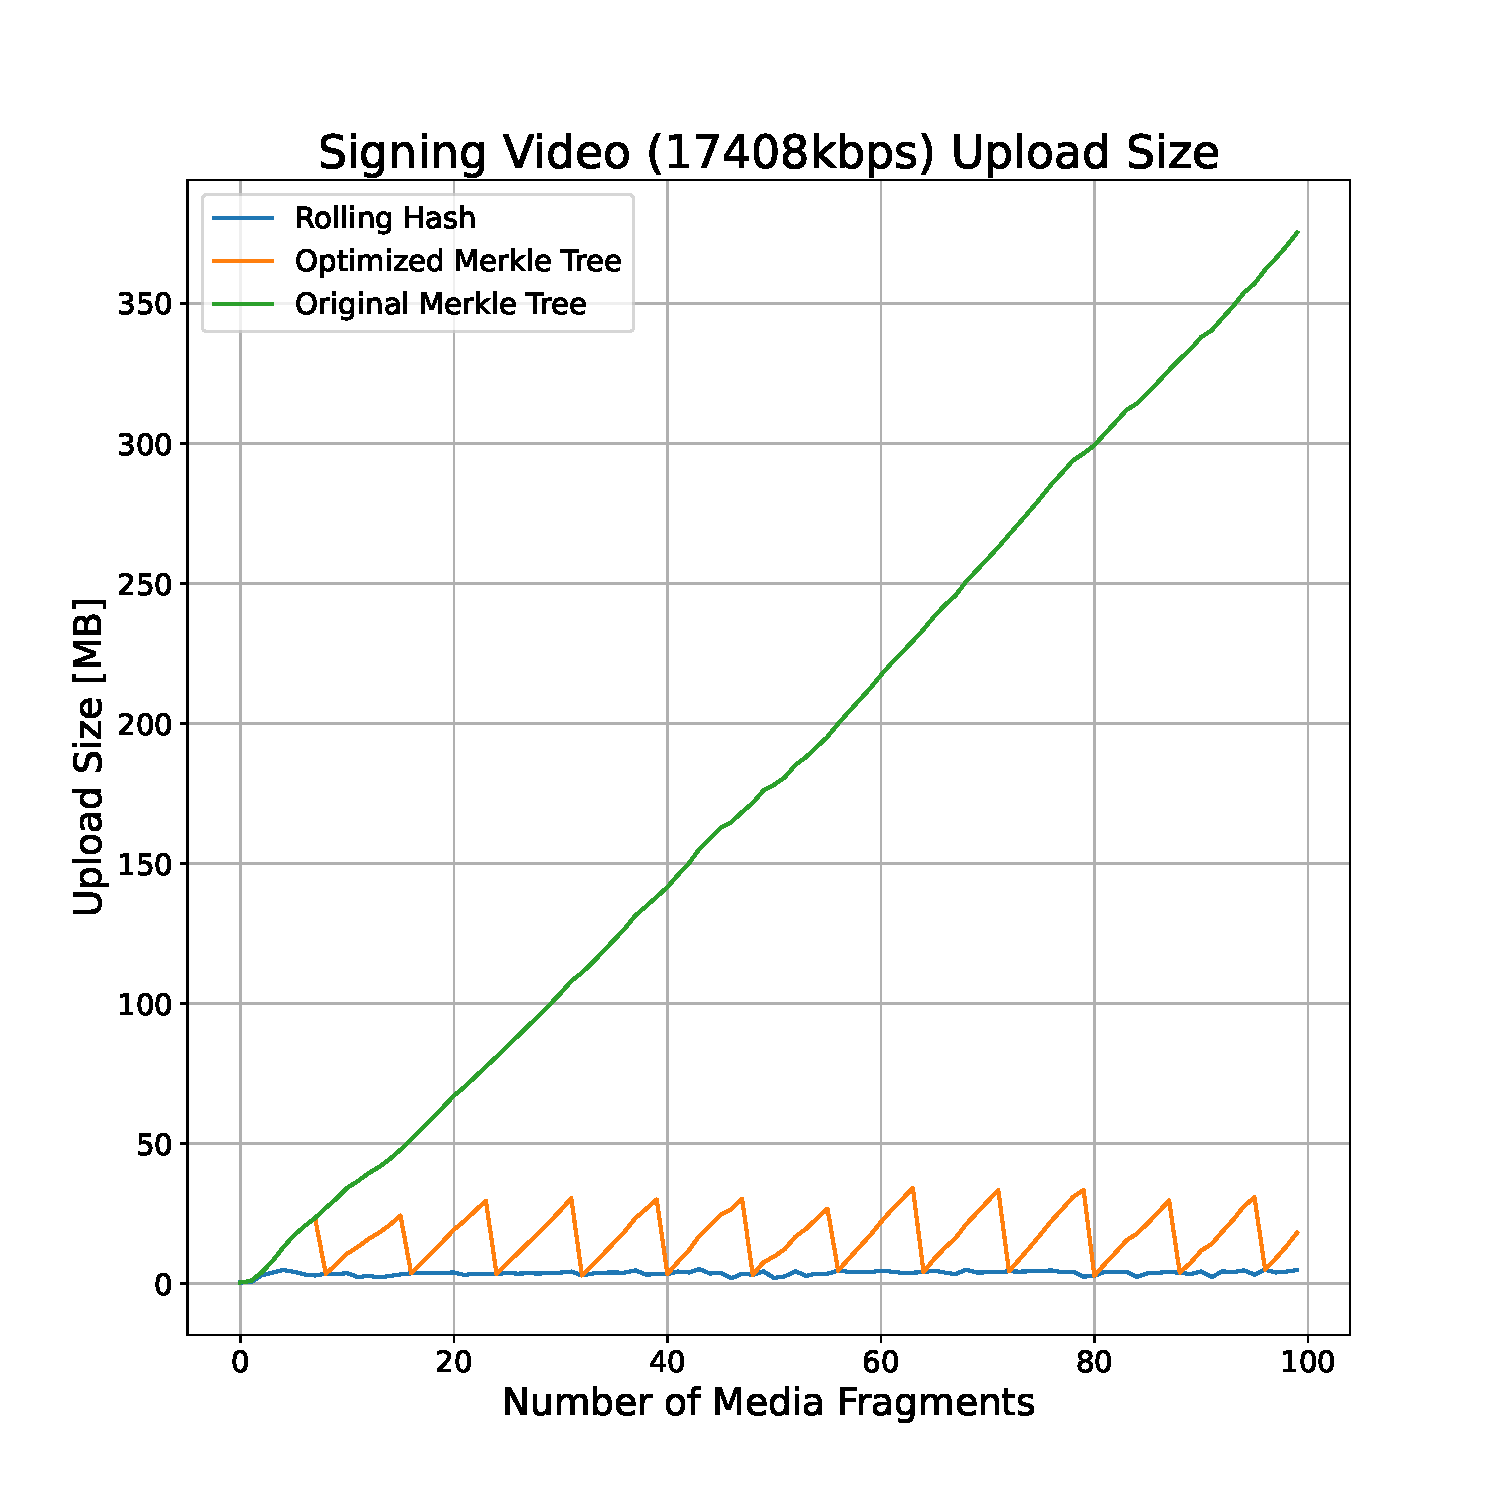
\includegraphics[width=0.49\linewidth]{plots/compare-upload-Video-(17408kbps).pdf}
        \label{fig:upload2-video3}
    }
    \caption{Upload Size Results}
    \label{fig:upload2}
\end{figure}

